\documentclass[psamsfonts, 12pt]{amsart}
%
%-------Packages---------
%
\usepackage[h margin=1 in, v margin=1 in]{geometry}
\usepackage{amssymb,amsfonts}
\usepackage[all,arc]{xy}
\usepackage{tikz-cd}
\usepackage{enumerate}
\usepackage{mathrsfs}
\usepackage{amsthm}
\usepackage{mathpazo}
\usepackage{float}
\usepackage[backend=biber]{biblatex}
\addbibresource{bibliography.bib}
%\usepackage{charter} %another font
%\usepackage{eulervm} %Vakil font
\usepackage{yfonts}
\usepackage{mathtools}
\usepackage{enumitem}
\usepackage{mathrsfs}
\usepackage{fourier-orns}
\usepackage[all]{xy}
\usepackage{hyperref}
\usepackage{url}
\usepackage{mathtools}
\usepackage{graphicx}
\usepackage{pdfsync}
\usepackage{mathdots}
\usepackage{calligra}
\usepackage{import}
\usepackage{xifthen}
\usepackage{pdfpages}
\usepackage{transparent}

\newcommand{\incfig}[2]{%
    \fontsize{48pt}{50pt}\selectfont
    \def\svgwidth{\columnwidth}
    \scalebox{#2}{\input{#1.pdf_tex}}
}
%
\usepackage{tgpagella}
\usepackage[T1]{fontenc}
%
\usepackage{listings}
\usepackage{color}

\definecolor{dkgreen}{rgb}{0,0.6,0}
\definecolor{gray}{rgb}{0.5,0.5,0.5}
\definecolor{mauve}{rgb}{0.58,0,0.82}

\lstset{frame=tb,
  language=Matlab,
  aboveskip=3mm,
  belowskip=3mm,
  showstringspaces=false,
  columns=flexible,
  basicstyle={\small\ttfamily},
  numbers=none,
  numberstyle=\tiny\color{gray},
  keywordstyle=\color{blue},
  commentstyle=\color{dkgreen},
  stringstyle=\color{mauve},
  breaklines=true,
  breakatwhitespace=true,
  tabsize=3
  }
%
%--------Theorem Environments--------
%
\newtheorem{thm}{Theorem}[section]
\newtheorem*{thm*}{Theorem}
\newtheorem{cor}[thm]{Corollary}
\newtheorem{prop}[thm]{Proposition}
\newtheorem{lem}[thm]{Lemma}
\newtheorem*{lem*}{Lemma}
\newtheorem{conj}[thm]{Conjecture}
\newtheorem{quest}[thm]{Question}
%
\theoremstyle{definition}
\newtheorem{defn}[thm]{Definition}
\newtheorem*{defn*}{Definition}
\newtheorem{defns}[thm]{Definitions}
\newtheorem{con}[thm]{Construction}
\newtheorem{exmp}[thm]{Example}
\newtheorem{exmps}[thm]{Examples}
\newtheorem{notn}[thm]{Notation}
\newtheorem{notns}[thm]{Notations}
\newtheorem{addm}[thm]{Addendum}
\newtheorem{exer}[thm]{Exercise}
%
\theoremstyle{remark}
\newtheorem{rem}[thm]{Remark}
\newtheorem*{claim}{Claim}
\newtheorem*{aside*}{Aside}
\newtheorem*{rem*}{Remark}
\newtheorem*{hint*}{Hint}
\newtheorem*{note}{Note}
\newtheorem{rems}[thm]{Remarks}
\newtheorem{warn}[thm]{Warning}
\newtheorem{sch}[thm]{Scholium}
%
%--------Macros--------
\renewcommand{\qedsymbol}{$\blacksquare$}
\renewcommand{\sl}{\mathfrak{sl}}
\newcommand{\Bord}{\mathsf{Bord}}
\renewcommand{\hom}{\mathsf{Hom}}
\renewcommand{\emptyset}{\varnothing}
\renewcommand{\O}{\mathscr{O}}
\newcommand{\R}{\mathbb{R}}
\newcommand{\ib}[1]{\textbf{\textit{#1}}}
\newcommand{\Q}{\mathbb{Q}}
\newcommand{\Z}{\mathbb{Z}}
\newcommand{\N}{\mathbb{N}}
\newcommand{\C}{\mathbb{C}}
\newcommand{\A}{\mathbb{A}}
\newcommand{\F}{\mathbb{F}}
\newcommand{\M}{\mathcal{M}}
\newcommand{\dbar}{\overline{\partial}}
\newcommand{\zbar}{\overline{z}}
\renewcommand{\S}{\mathbb{S}}
\newcommand{\V}{\vec{v}}
\newcommand{\RP}{\mathbb{RP}}
\newcommand{\CP}{\mathbb{CP}}
\newcommand{\B}{\mathcal{B}}
\newcommand{\GL}{\mathsf{GL}}
\newcommand{\SL}{\mathsf{SL}}
\newcommand{\SP}{\mathsf{SP}}
\newcommand{\SO}{\mathsf{SO}}
\newcommand{\SU}{\mathsf{SU}}
\newcommand{\gl}{\mathfrak{gl}}
\newcommand{\g}{\mathfrak{g}}
\newcommand{\Bun}{\mathsf{Bun}}
\newcommand{\inv}{^{-1}}
\newcommand{\bra}[2]{ \left[ #1, #2 \right] }
\newcommand{\set}[1]{\left\lbrace #1 \right\rbrace}
\newcommand{\abs}[1]{\left\lvert#1\right\rvert}
\newcommand{\norm}[1]{\left\lVert#1\right\rVert}
\newcommand{\transv}{\mathrel{\text{\tpitchfork}}}
\newcommand{\defeq}{\vcentcolon=}
\newcommand{\enumbreak}{\ \\ \vspace{-\baselineskip}}
\let\oldexists\exists
\renewcommand\exists{\oldexists~}
\let\oldL\L
\renewcommand\L{\mathfrak{L}}
\makeatletter
\newcommand{\tpitchfork}{%
  \vbox{
    \baselineskip\z@skip
    \lineskip-.52ex
    \lineskiplimit\maxdimen
    \m@th
    \ialign{##\crcr\hidewidth\smash{$-$}\hidewidth\crcr$\pitchfork$\crcr}
  }%
}
\makeatother
\newcommand{\bd}{\partial}
\newcommand{\lang}{\begin{picture}(5,7)
\put(1.1,2.5){\rotatebox{45}{\line(1,0){6.0}}}
\put(1.1,2.5){\rotatebox{315}{\line(1,0){6.0}}}
\end{picture}}
\newcommand{\rang}{\begin{picture}(5,7)
\put(.1,2.5){\rotatebox{135}{\line(1,0){6.0}}}
\put(.1,2.5){\rotatebox{225}{\line(1,0){6.0}}}
\end{picture}}
\DeclareMathOperator{\id}{id}
\DeclareMathOperator{\im}{Im}
\DeclareMathOperator{\codim}{codim}
\DeclareMathOperator{\coker}{coker}
\DeclareMathOperator{\supp}{supp}
\DeclareMathOperator{\inter}{Int}
\DeclareMathOperator{\sign}{sign}
\DeclareMathOperator{\sgn}{sgn}
\DeclareMathOperator{\indx}{ind}
\DeclareMathOperator{\alt}{Alt}
\DeclareMathOperator{\Aut}{Aut}
\DeclareMathOperator{\trace}{trace}
\DeclareMathOperator{\ad}{ad}
\DeclareMathOperator{\End}{End}
\DeclareMathOperator{\Ad}{Ad}
\DeclareMathOperator{\Lie}{Lie}
\DeclareMathOperator{\spn}{span}
\DeclareMathOperator{\dv}{div}
\DeclareMathOperator{\grad}{grad}
\DeclareMathOperator{\Sym}{Sym}
\DeclareMathOperator{\sheafhom}{\mathscr{H}\text{\kern -3pt {\calligra\large om}}\,}
\newcommand*\myhrulefill{%
   \leavevmode\leaders\hrule depth-2pt height 2.4pt\hfill\kern0pt}
\newcommand\niceending[1]{%
  \begin{center}%
    \LARGE \myhrulefill \hspace{0.2cm} #1 \hspace{0.2cm} \myhrulefill%
  \end{center}}
\newcommand*\sectionend{\niceending{\decofourleft\decofourright}}
\newcommand*\subsectionend{\niceending{\decosix}}
\def\upint{\mathchoice%
    {\mkern13mu\overline{\vphantom{\intop}\mkern7mu}\mkern-20mu}%
    {\mkern7mu\overline{\vphantom{\intop}\mkern7mu}\mkern-14mu}%
    {\mkern7mu\overline{\vphantom{\intop}\mkern7mu}\mkern-14mu}%
    {\mkern7mu\overline{\vphantom{\intop}\mkern7mu}\mkern-14mu}%
  \int}
\def\lowint{\mkern3mu\underline{\vphantom{\intop}\mkern7mu}\mkern-10mu\int}
%
%--------Hypersetup--------
%
\hypersetup{
    colorlinks,
    citecolor=black,
    filecolor=black,
    linkcolor=blue,
    urlcolor=blacksquare
}
%
%--------Solution--------
%
\newenvironment{solution}
  {\begin{proof}[Solution]}
  {\end{proof}}
%
%--------Graphics--------
%
%\graphicspath{ {images/} }

\begin{document}
%
\author{Jeffrey Jiang}
%
\title{A (Not so) Quick Survey of Hodge Theory}
%
\maketitle
%
These are some notes I typed up reading through Voisin's text \emph{Hodge Theory
and Complex Algebraic Geometry, I}, with some supplemental details coming Daniel
Huybrechts' \emph{Complex Geometry}. The structure of the notes mostly follows Voisin,
with some added details included for my own sake.
%
\tableofcontents
%
\section{Linear Algebra}
%
\begin{defn}
Let $V$ be a finite dimensional $\R$-vector space. An \ib{almost complex structure} on
$V$ is a linear map $J : V \to V$ satisfying $J^2 = \id_V$. An \ib{almost complex
vector space} is tuple $(V,J)$, where $V$ is a finite dimensional $\R-$vector space
equipped with an almost complex structure $J$.
\end{defn}
%
The data of an almost complex structure $J$ is equivalent to giving $V$ the structure
of a complex vector space, where we define $(a + bi)\cdot v = ab + bJv$. Because of this,
we may call $J$ a \ib{complex structure}. We use the name \emph{almost} complex
structure to emphasize the differences between the analogous constructions in the
nonlinear world of manifolds. Note that since an almost complex structure is equivalent
to a complex structure, this immediately implies that $V$ is even dimensional. \\

One way to think about an almost complex structure is through the geometric
interpretation of complex multiplication. If we regard $\C$ as a $2$-dimensional vector
space over $\R$, multiplication by $i$ corresponds to a rotation by $\pi/2$ in the
counterclockwise direction, and multiplication by $-i$ corresponds to a rotation by
$\pi/2$ in the clockwise direction. From this we see that a choice of a square root
of $-1$ comes with a choice of clockwise or counterclockwise. This implies that
every complex vector space is canonically oriented as a real vector space. Given a
$\C$-vector space $V$ with $\C$-basis $\set{z_1, \ldots, z_n}$, we have that the ordered
basis $(z_1, iz_1, \ldots z_n, iz_n)$ defines a positively oriented basis for $V$ over
$\R$.
%
\begin{defn}
Let $V$ by any $\R$-vector space. The \ib{complexification} of $V$ is the complex
vector space $V_\C = \C \otimes_\R V$. The complexification $V_\C$ is naturally a
complex vector space, where for $\lambda \in \C$, the action of $\lambda$ on a
homogeneous element $\mu \otimes v$ is given by
\[
\lambda \cdot (\mu \otimes v) = \lambda\mu \otimes v
\]
\end{defn}
%
The complexification is a different way of obtaining a complex vector space from a real
one. The complexification $V_\C$ is a vector space of twice the dimension of $V$ as a
vector space over $\R$. In addition, there is a natural inclusion
$V \hookrightarrow V_\C$ given by $v \mapsto 1 \otimes v$. Complexification is an
instance of \emph{extension of scalars} -- every element of $V_\C$ is of the form
$av + biw$ where $a,b \in \R$, and $v,w \in V$. Therefore, we will denote the element
$(a + bi) \otimes v \in V_\C$ by $av + biv$, and we have a direct sum decomposition
$V_\C = V \oplus iV$.   Given a linear map $T : V \to W$ of $\R$-vector spaces, we can
extend $T$ to a complexified map $T_\C : V_\C \to W_\C$, where
$T_\C(av + biw) = aTv + biTv$. In other words, $T_\C = \id_\C \otimes T$. In this way,
we see that complexification defines a covariant functor
$\mathsf{Vect}_\R \to \mathsf{Vect}_\C$ from the category of $\R$-vector spaces to the
category of $\C$-vector spaces. \\

A natural question to ask is how an almost complex structure interacts with
the process of complexification. Let $(V,J)$ be an almost complex vector space. Then the
complexified map $J_\C : V_\C \to V_\C$ squares to $-1$, and admits eigenvalues
$\pm i$. For example, consider $V = \C$. We then can then make the natural
identification of $\C$ with the almost complex vector space $(\R^2, J)$, where $J$
is given by the matrix
\[
J = \begin{pmatrix}
0 & -1 \\
1 & 0
\end{pmatrix}
\]
using the ordered $\R$ basis $(1,i)$. Then $V_\C = \C \otimes_\R \C = \C^2$, and $J_\C$
is given by the matrix
\[
J_\C = \begin{pmatrix}
0 & -1 & 0 & 0 \\
1 & 0 & 0 & 0 \\
0 & 0 & 0 & -1 \\
0 & 0 & 1 & 0
\end{pmatrix}
\]
in the ordered $\R$ basis $(1, i, 1, i)$, where the first pair elements are elements of
one copy of $\C^2$, and the second pair of elements are elements of a separate copy of
$\C^2$, giving an $\R$ basis for $\C \cong \C \oplus \C$. The matrix $J_\C$
clearly has eigenvalues $\pm i$, with the $i$-eigenspace being spanned by the
vectors
\[
\begin{pmatrix}
\frac{1}{2} \\[5pt]
0 \\[5pt]
\frac{1}{2} \\[5pt]
0
\end{pmatrix}, \begin{pmatrix}
\frac{i}{2} \\[5pt]
0 \\[5pt]
-\frac{i}{2} \\[5pt]
0
\end{pmatrix}
\]
and the $-i$ eigenspace being the span of
\[
\begin{pmatrix}
0 \\[5pt]
\frac{1}{2} \\[5pt]
0 \\[5pt]
\frac{1}{2}
\end{pmatrix}, \begin{pmatrix}
0 \\[5pt]
\frac{i}{2} \\[5pt]
0 \\[5pt]
-\frac{i}{2}
\end{pmatrix}
\]
The case for general $V$ is similar, and amounts to fixing an $\R$ basis of the
form $\set{v_1, Jv_1, \ldots v_n, Jv_n}$ for $(V,J)$. The decomposition of $V_\C$ into
the $\pm i$-eigenspaces of $J_\C$ gives a direct sum decomposition
\[
V_\C = V^{1,0} \oplus V^{0,1}
\]
where $V^{1,0}$ denotes the $i$-eigenspace, and $V^{0,1}$ denotes the $-i$-eigenspace.
Note that in the bases we chose above for $\C^2$, complex conjugation is given by the
matrix
\[
\begin{pmatrix}
0 & 1 & 0 & 0\\
1 & 0 & 0 & 0 \\
0 & 0 & 0 & 1 \\
0 & 0 & 1 & 0
\end{pmatrix}
\]
and determines an isomorphism of complex vector spaces
$V^{1,0} \cong \overline{V^{0,1}}$ and vice versa. In addition, complex conjugation
picks out a distinguished subspace of $V_\C$ isomorphic to $V$ -- the $1$-eigenspace.
Elements of this eigenspace are called \ib{real} (much like how the $\R^n$
is left invariant under complex conjugation in $\C^n$). \\

An almost complex structure $J$ on $V$ induces a dual map $J^* : V^* \to V^*$. By
functoriality of taking dual spaces, $(J^*) ^2 = -\id_{V^*}$, giving $V^*$ the
structure of an almost complex vector space via $J^*$. Explicitly, given a linear
functional $\alpha \in V^*$, we have that the action of $J^*$ on $\alpha$ is given
by
\[
(J^*\alpha)(v) = \alpha(Jv)
\]
for every $v \in V$. We then get an analogous decomposition of the complexified
dual space$ V^*_\C = \hom_\R(V,\C)$ as
\[
V^*_\C = (V^*)^{1,0} \oplus (V^*)^{0,1}
\]
into the $\pm i$ eigenspaces of $J^*$, which have very natural interpretations in
terms of $V$. The subspace $(V^*)^{1,0}$ consists of the $\alpha$ such that
$\alpha(Jv) = i\alpha(v)$. We have a natural pairing
 $(V^*)^{1,0} \otimes V^{1,0} \to \C$
given by
\[
\langle \alpha,v \rangle = \alpha(v)
\]
which is nondegenerate, establishing the two vector spaces as dual to each other (as
complex vector spaces). A similar statement holds for $V^{0,1}$ and $(V^*)^{0,1}$,
putting them in duality as well. Another perspective to take is that the condition
that $\alpha(Jv) = i\alpha(v)$ is equivalent to $\alpha$ being \emph{complex linear}
with respect to the complex structure $J$ on $V$ and $i$ on $\C$, giving us an
isomorphism $(V^*)^{1,0} \cong \hom_\C(V,\C)$. Similarly, we have that
$(V^*)^{0,1} \cong \hom_{\C}(V,\overline{\C})$.\\

We the consider the effects of complexification on another linear algebraic construction
--the exterior algebra. Given a finite dimensional $\R$-vector space $V$, we have that
the exterior algebra $\Lambda^\bullet V$ has a natural $\Z$-grading
\[
\Lambda^\bullet V = \bigoplus_{k = 0}^n \Lambda^kV
\]
Upon complexification, we have a canonical isomorphism
$(\Lambda^\bullet V)_\C \cong \Lambda^\bullet V_\C$, where the right hand side is the
exterior algebra of $V_\C$ as a \emph{complex} vector space
(i.e. $\Lambda^0 V_\C \cong \C$, not $\R$), and $\Lambda^\bullet V$ is canonically
embedded in $\Lambda^\bullet V_\C$ as the subspace invariant under complex conjugation.
Further assume that we have an almost complex structure $J : V \to V$. This gives a
direct sum decomposition $V_\C = V^{1,0} \oplus V^{0,1}$, which then induces a
decomposition
\[
\Lambda^kV_\C \cong \bigoplus_{p+q=k}\Lambda^pV^{1,0} \otimes_\C \Lambda^q V^{0,1}
\]
giving the complexified exterior algebra a bigrading via the subspaces
\[
\Lambda^{p,q}V \defeq \Lambda^p V^{1,0} \otimes_\C \Lambda^q V^{0,1}
\]
elements of $\Lambda^{p,q}$ are said to have \ib{bidegree} $(p,q)$. We now make several
simple observations regarding the bigrading of $\Lambda^\bullet V_\C$, which stem from
our observations regarding the decomposition $V_\C = V^{1,0} \oplus V^{0,1}$.
%
\begin{enumerate}
  \item From the fact that $\overline{V^{1,0}} = V^{0,1}$, we get that
  $\overline{\Lambda^{p,q}V} = \Lambda^{q,p}V$.
  \item Given $\omega \in \Lambda^{p,q}V$ and $\eta \in \Lambda^{s,t}V$, we have that
  $\omega \wedge \eta \in \Lambda^{p+s,q+t}V$.
\end{enumerate}
%
\section{Complex Manifolds}
%
We now transfer our linear algebraic knowledge to complex manifolds. Let $U \subset \C$
be an open subset, and $z = x + iy$ the usual coordinate function on $U$. Considered
as a subset of $\R^2$, for any point $p \in U$, the tangent space $T_pU$ is spanned by
the coordinate vectors $\partial_x\vert_p$ and $\partial_y\vert_p$. If we then
complexify, the $\partial_x\vert_p$ and $\partial_y\vert_p$ also form a basis for
$(T_pU)_\C$ as a \emph{complex} vector space. Consequently, we can also form a
basis for $(T_pU)_\C$ with the vectors
%
\begin{align*}
\frac{\partial}{\partial z}\bigg\vert_p &\defeq
\frac{1}{2}\left(\frac{\partial}{\partial x} - i\frac{\partial}{\partial y}\right) \\
\frac{\partial}{\partial\overline{z}}\bigg\vert_p &\defeq
\frac{1}{2}\left( \frac{\partial}{\partial x} + i\frac{\partial}{\partial y}\right)
\end{align*}
%
which we abbreviate as $\partial_z\vert_p$ and $\partial{\overline{z}}\vert_p$
respectively. Doing this for all $p$, we obtain vector fields $\partial_z$ and
$\partial_{\overline{z}}$ on all of $U$, where a function $f \in C^\infty(U, \C)$ is
holomorphic if and only if $\partial_{\overline{z}}f = 0$. Functions $f$ annihilated by
$\partial_z$ are \ib{antiholomorphic}, i.e. $\overline{f}$ is holomorphic. These
vector fields give a framing for the complexified tangent bundle $TU_\C$, i.e. an
isomorphism $TU_\C \to U \times \C^2$. \\

We get a similar description of the complexified cotangent bundle $T^*U_\C$, which
is framed by the covector fields
%
\begin{align*}
dz = \frac{1}{2}\left(dx + idy\right) \\
d\overline{z} = \frac{1}{2}\left( dx -idy\right)
\end{align*}
%
which are easily verified to the duals of $\partial_z$ and $\partial_{\overline{z}}$
respectively. For an open subset $U \subset \C^n$ with complex coordinates
$z^i = x^i +iy^i$, we have analogous vector fields $\partial/\partial z^i$ and
$\partial/\partial\overline{z}^i$ and covector fields $dz^i$ and $d\overline{z}^i$.
%
\begin{defn}
An \ib{almost complex manifold} is the data of a smooth manifold $X$ and a smooth
section $J \in \Gamma_X(\End(TX))$ such that $J^2 = -\id_{TX}$.
\end{defn}
%
\begin{defn}
A \ib{complex manifold} is a smooth manifold $X$ such that there is an open cover
$\set{(U_\alpha, \varphi_\alpha)}$ of $X$ by charts $U_\alpha$ and diffeomorphisms
$\varphi: U_\alpha \to V_\alpha$ to open sets $V_\alpha \subset \R^{2n} \cong \C^n$
such that the transition maps $\varphi_\alpha \circ \varphi_\beta\inv$ are holomorphic.
\end{defn}
%
\begin{defn}
Let $X$ be a complex manifold. A complex valued function $f \in C^\infty(X,\C)$ is
\ib{holomorphic} if for any holomorphic chart $(\varphi, U)$, we have that
$f \circ \varphi\inv$ is holomorphic. The ring of holomorphic functions over $X$ is
denoted $\O_X$.
\end{defn}
%
Unlike the linear case, the notion of an almost complex manifold and a complex manifold
are \emph{not} equivalent. Let $(X,J)$ be an almost complex manifold. For a point
$x \in X$, we have that $J_x$ is an almost complex structure on the tangent space
$T_xX$, which gives a decomposition of the complexified tangent space
\[
T_xX_\C = T_x^{1,0}X \oplus T_x^{0,1}X
\]
into the $\pm i$-eigenspaces of complexified $J_x$. Doing this over all points $x$,
we get a decomposition of the complexified tangent bundle
\[
TX_\C = T^{1,0}X \oplus T^{0,1}X
\]
into the $\pm i$-eigenbundles of $J$.\\

Suppose $X$ is a complex manifold. Then every tangent space $T_xX$ inherits an almost
complex structure coming from multiplication by $i$ in $\C^n$, giving an almost complex
structure $J$ on $X$. To show this explicitly, let $z^i = x^i + iy^i$ be local
holomorphic coordinates for $X$. Then the coordinate functions
$(x^1, y^1, \ldots x^n, y^n)$ form a coordinate system for $X$ as a \emph{real} manifold,
and the action of $J$ in these coordinates is simply given by
%
\begin{align*}
\frac{\partial}{\partial x^i} &\mapsto \frac{\partial}{\partial y^i} \\
\frac{\partial}{\partial y^i} &\mapsto -\frac{\partial}{\partial x^i}
\end{align*}
%
and the subbundle $T^{1,0}X \subset TX_\C$ is spanned by the $\partial/\partial z^i$,
and $T^{0,1}X$ is spanned by the $\partial/\partial\overline{z}^i$. The composition
\[\begin{tikzcd}
TX \ar[r,hookrightarrow] & TX_\C \ar[r] & T^{1,0}X
\end{tikzcd}\]
consisting of the inclusion followed by projecting then defines an isomorphism of
the real tangent bundle with $T^{1,0}X$, which is called the
\ib{holomorphic tangent bundle}. Explicitly, this map is given in local coordinates by
%
\begin{align*}
\frac{\partial}{\partial x^i} &=
\frac{\partial}{\partial z^i} + \frac{\partial}{\partial\overline{z}^i}
\mapsto \frac{\partial}{\partial z^i} \\
\frac{\partial}{\partial y^i} &=
i\frac{\partial}{\partial z^i} - i\frac{\partial}{\partial\overline{z}^i}
\mapsto i\frac{\partial}{\partial z^i}
\end{align*}
%
and the $\partial/\partial z^i$ along with the $i\partial/\partial z^i$ form a local
frame for the holomorphic tangent bundle $T^{1,0}X$.\\

Given an almost complex manifold $(X,J)$, a natural question to ask is whether or not
$X$ admits the structure of a complex manifold where $J$ is multiplication by $i$.
The answer to this question is a celebrated theorem of Newlander and Nirenberg
%
\begin{thm}[\ib{Newlander-Nirenberg}]
An almost complex manifold $(X,J)$ is a complex manifold (where $J$ is multiplication by
$i$) if and only if the subbundle $T^{1,0}X \subset TX_\C$ is integrable in the sense
of Frobenius, i.e.
\[
[T^{1,0}X, T^{1,0}X] \subset T^{1,0}X
\]
via complex conjugation, this is equivalent to $T^{0,1}X$ being integrable.
\end{thm}
%
Intuitively, the existence of local \emph{holomorphic} coordinates amounts to
finding an integral submanifold for $T^{1,0}X$, since if $X$ was complex, $T^{1,0}X$
would arise as the holomorphic tangent bundle of $X$.
%
\section{Cohomology of Complex Manifolds.}
%
Let $X$ be a complex manifold, and let $J$ denote the canonical almost complex structure
on $X$. Applying our linear algebraic knowledge pointwise, we get a decomposition of
the complexified cotangent bundle
\[
T^*X_\C = (T^*X)^{1,0} \oplus (T^*X)^{0,1}
\]
%
which then gives a decomposition of the space $\Omega^k_X(\C)$ of complex valued
differential $k$-forms as
\[
\Omega^k_X(\C) = \bigoplus_{p+q=k}\Omega^{p,q}_X(\C)
\]
where $\Omega^{p,q}_X(\C)$ denotes the space of $(p,q)$-forms, i.e. sections of
$\Lambda^{p,q}T^*X$, and the direct sum is taken as modules over $C^\infty(X,\C)$.
Out of all the $\Lambda^{p,q}T^*X$, there is a distinguished bundle.
%
\begin{defn}
Let $X$ be a complex manifold of complex dimension $\dim_\C X = n$ (i.e. $\dim X = 2n)$.
The \ib{canonical bundle} of $X$, denote $K_X$, is the complex vector bundle
\[
K_X = \Lambda^{n,0}T^*X
\]
\end{defn}
%
Let $d$ denote the de Rham differential $\Omega^k_X \to \Omega^{k+1}_X$ after
complexifying it to obtain a map $\Omega^k_X(\C) \to \Omega^{k+1}_X(\C)$. In local
holomorphic coordinates $\set{z^i}$, we have that the $dz^i$ form a basis for the space
of smooth $(1,0)$-forms over the ring $C^\infty(M,\C)$, and the $d\overline{z}^i$ form a
basis for the space of smooth $(0,1)$-forms. Therefore, given $f \in C^\infty(X,\C)$, we
can uniquely write $df \in \Omega^1_X(\C)$ as
\[
df = \frac{\partial f}{\partial z^i}dz^i +
\frac{\partial f}{\partial\overline{z}^i}d\overline{z}^i
\]
where we use Einstein summation notation. Given an arbitrary $(p,q)$ form $\alpha$, it
has the local coordinate expression
\[
\alpha = \sum_{p,q} \alpha_{p,q} dz^{i_1} \wedge \ldots \wedge dz^{i_p} \wedge
d\overline{z}^{i_1}\ldots \wedge d\overline{z}^{i_q}
\]
for smooth $\alpha_{p,q} \in C^\infty(X,\C)$. Then we have that
%
\begin{align*}
d\alpha &= \left(\sum_{p,q}\frac{\partial\alpha_{p,q}}{\partial z^i} dz^i
\wedge dz^{i_1} \wedge \ldots \wedge dz^{i_p} \wedge
d\overline{z}^{i_1}\ldots \wedge d\overline{z}^{i_q}\right) \\[5pt]
&+ \left(
\sum_{p,q}\frac{\partial\alpha_{p,q}}{\partial \overline{z}^i} d\overline{z}^i
\wedge dz^{i_1} \wedge \ldots \wedge dz^{i_p} \wedge
d\overline{z}^{i_1}\ldots \wedge d\overline{z}^{i_q}
\right)
\end{align*}
%
which shows that $d\alpha$ is a $(p+1,q+1)$ form, i.e. $d$ is of bidegree $(1,1)$. This
expression for $d\alpha$ allows us to decompose $d$ as a sum $d = \partial + \dbar$,
where
%
\begin{align*}
\partial\alpha &= \sum_{p,q}\frac{\partial\alpha_{p,q}}{\partial z^i} dz^i
\wedge dz^{i_1} \wedge \ldots \wedge dz^{i_p} \wedge
d\overline{z}^{i_1}\ldots \wedge d\overline{z}^{i_q} \\[5pt]
\dbar\alpha &= \sum_{p,q}\frac{\partial\alpha_{p,q}}{\partial \overline{z}^i}
d\overline{z}^i \wedge dz^{i_1} \wedge \ldots \wedge dz^{i_p} \wedge
d\overline{z}^{i_1}\ldots \wedge d\overline{z}^{i_q}
\end{align*}
%
from the definition, it is clear that $\partial$ is of bidegree $(1,0)$ and $\dbar$ is
of bidegree $(0,1)$.
%
\begin{prop}\enumbreak
\begin{enumerate}
  \item $\partial^2 = 0$
  \item $\dbar^2 = 0$
  \item $\partial\dbar + \dbar\partial = 0$
\end{enumerate}
\end{prop}
%
\begin{proof}
We know that $d = \partial + \dbar$ satisfies $d^2 = 0$. Therefore, we have that
\[
d^2 = (\partial +\dbar)^2 = \partial^2 + \partial\dbar + \dbar\partial + \dbar^2
\]
we then note that the bidegrees of all the components. We have:
\begin{enumerate}
  \item $\partial^2$ has bidegree $(2,0)$.
  \item $\partial\dbar + \dbar\partial$ has bidegree $(1,1)$
  \item $\dbar^2$ has bidegree $(0,2)$
\end{enumerate}
in order for $d^2$ to vanish, all the terms of different bidegrees must vanish, proving
all three parts of the proposition.
\end{proof}
%
The operators $\partial$ and $\dbar$ satisfy many of the same identities as $d$. Another
helpful identity to note is that
\[
\partial\alpha = \overline{\dbar\overline{\alpha}}
\]
\begin{defn}
Let $X$ be a complex manifold. A \ib{holomorphic vector bundle} over $X$ is a
complex vector bundle $\pi : E \to X$ such that the total space $E$ is a complex
manifold
and the projection $\pi$ is a holomorphic map.
\end{defn}
%
\begin{exmp}
For a complex manifold $X$, the complex vector bundles $\Lambda^{q,0}T^*X$ are all
holomorphic vector bundles, which is easily seen using local trivializations defined
by local holomorphic coordinates.
\end{exmp}
%
Note again that a holomorphic vector bundle is \emph{not} a complex vector bundle
(for example, a complex vector bundle can be odd dimensional if the base space is
odd dimensional). Instead, it is a complex bundle with extra structure. Let
$\sigma : X \to E$ be a \emph{smooth} section. In a local holomorphic trivialization of
$E$, we can write $\sigma$ as
\[
\sigma = (\sigma^1, \ldots, \sigma^k)
\]
for smooth complex-valued functions $\sigma^i$,  where $k$ is the rank of $E$ as a
complex vector bundle. In this trivialization, we can apply the operator $\dbar$
component-wise to get
\[
\dbar\sigma = (\dbar\sigma^1,\ldots,\dbar\sigma^k)
\]
and this local definition glues together to give a well defined operator
$\dbar_E : \Omega^{0,0}_X(E) \to \Omega^{0,1}_X(E)$, where $\Omega^{p,q}_X(E)$ denotes
the space of sections $\Gamma_X(T^{p,q}X \otimes_\C E)$. We then note that the
holomorphic sections $X \to E$ are exactly those annihilated by $\dbar_E$. Since
$\dbar_E$ is defined locally in terms of $\dbar$, we immediately see that
$\dbar_E^2 = 0$, giving us the
\ib{Dolbeault complex} of $E$.
\[\begin{tikzcd}
\Omega^{0,0}_X(E) \ar[r, "\dbar_E"] & \Omega^{0,1}_X(E) \ar[r, "\dbar_E"] &
\cdots\cdots \ar[r, "\dbar_E"] & \Omega^{0,n}_X(E) \ar[r,"\dbar_E"] & 0
\end{tikzcd}\]
%
The \ib{Dolbeault cohomology groups} of $E$ are the cohomology groups of the
Dolbeault complex, and are denoted $H^p(X,E)$. In the case $E = \Lambda^{0,q}T^*X$,
we have that $\dbar_E = \dbar$, and we denote these cohomology groups by
\[
H^{p,q}(X) = H^p(X,\Lambda^{0,q}T^*X)
\]
%
\section{K\"ahler Manifolds}
%
K\"ahler manifolds will form a special class of manifolds where Hodge theory
will prove especially useful. Before diving into the world of K\"ahler manifolds,
we do some prerequisite linear algebra, which is closely tied to Hermitian geometry.
%
\begin{defn}
Let $V$ be a complex vector space. A \ib{Hermitian form} on $V$ is a bilinear map
$h : \overline{V} \otimes_\C V \to \C$ satisfying $h(v,w) = \overline{h(w,v)}$.
\end{defn}
%
Another way to define a Hermitian form is as a \ib{sesquilinear} form
$h : V \otimes_\C V \to \C$, i.e. conjugate linear in the first term, and linear in the
second term, along with the Hermitian symmetry condition $h(v,w) = \overline{h(v,w)}$.
In a basis for $V$, a Hermitian form is given by a Hermitian matrix $H$, i.e.
$H^\dagger = H$. \\

Given a Hermitian form $h$ on a complex vector space $V$, we can decompose $h$ into
its real and imaginary parts. Let $g = \mathfrak{Re}(h)$ and
$\omega = \mathfrak{Im}(h)$, so we have $h = g + i\omega$.
%
\begin{prop}
Let $h = g + i\omega$ be a hermitian form. Then we have
\begin{enumerate}
  \item $g$ is symmetric
  \item $\omega$ is skew-symmetric
\end{enumerate}
\end{prop}
%
\begin{proof}\enumbreak
\begin{enumerate}
  \item Since $h$ is Hermitian, we have that $h(v,w) = \overline{h(w,v)}$, which have
  the same real part. Therefore, $g(v,w) = g(w,v)$, so $g$ is symmetric
  \item We again use the fact that $h(v,w) = \overline{h(w,v)}$. Since conjugation
  reverses the sign on the imaginary component, we immediately get that
  $\omega(v,w) = -\omega(w,v)$.
\end{enumerate}
\end{proof}
%
\begin{rem*}
The decomposition of $h$ into its real and imaginary components is one way of seeing
the useful identity
\[
U_n = O_{2n} \cap Sp_{2n} \cap GL_n\C
\]
where we regard all of the groups as subgroups of $GL_{2n}\R$. Any matrix preserving
the standard Hermitian form on $\C^n$ must necessarily preserve both the real and
imaginary components, so it must preserve the standard Euclidean inner product on
$\R^{2n} \cong \C^n$ and the standard symplectic form on $\R^{2n} \cong \C$.
\end{rem*}
%
Given a complex vector space $V$ equipped with a hermitian metric $h$, let $J$
denote the natural almost complex structure induced by multiplication by $i$.
Writing $h = g + i\omega$, we see that $\omega$ and $g$ are intimately related, i.e.
\begin{enumerate}
  \item $g(v,Iw) = \omega(v,w)$
  \item $\omega(v,Iw) = g(v,w)$
\end{enumerate}
%
both of which come from the fact that $h$ is compatible with $J$ in the sense that
$h(Jv,Jw) = h(v,w)$. Finally, we note that $\omega$ can be naturally identified
with a real element of $(V^*)^{1,1}$.
%
\begin{defn}
Let $h$ be a Hermitian form, and $\omega = \mathfrak{Im}(h)$. Then $\omega$ is called
the \ib{K\"ahler form} of $h$.
\end{defn}
%
We now move back to the world of manifolds. Let $(X,J)$ be an almost complex manifold.
The almost complex structure gives each tangent space $T_xX$ the structure of a complex
vector space, so it makes sense to discuss a Hermitian form $h_x$ on $T_xX$.
%
\begin{defn}
A \ib{K\"ahler manifold} is an almost complex manifold $(X,J)$ with a smoothly varying
Hermitian metric (i.e. a positive definite Hermitian form) $h$ where $J$ is integrable
and the K\"ahler form $\omega$ obtained from $h$ is closed.
\end{defn}
%
From the decomposition $h = g + i\omega$, we see that a K\"ahler manifold is a
melting pot of several compatible structures, namely the Riemannian metric $g$, the
almost complex structure $J$, and the symplectic form $\omega$. \\

From the basic definition, we can already make some surprisingly deep statements about
K\"ahler manifolds.
%
\begin{prop}
Let $X$ be a K\"ahler manifold with Hermitian form $h = g + i\omega$. Then the volume
form of $X$ with respect to the Riemannian metric $g$ is $\omega^n/n!$, where
$n = \dim_\C X$.
\end{prop}
%
\begin{proof}
It suffices to verify this pointwise for a fixed point $x \in X$.
The Riemannian volume form $dV_g$ is uniquely characterized by the fact that
$(dV_g)_x(e_1, \ldots, e_{2n}) = 1$ for an oriented orthonormal basis
$\set{e_1, \ldots e_{2n}}$ for $T_xX$. Arrange local holomorphic coordinates
$\set{z^i}$ about $x$ such that at $x$, the Hermitian form $h_x$ is given by the
identity matrix, i.e.
\[
h_x\left(\frac{\partial}{\partial z^i}\bigg\vert_x,
\frac{\partial}{\partial z^j}\bigg\vert_x\right) = \delta_{ij}
\]
Let $\partial_i$ denote $\partial/\partial z^i\vert_x$. We then have that
$\set{\partial_1, i\partial_1, \ldots \partial_n, i\partial_n}$ is an oriented
orthonormal $\R$-basis for $T_xX$ with respect to $g$, so it suffices to evaluate
$\omega^n_x$ on this basis, and verify that it evaluates to $n!$. To do this, we
use a lemma.
%
\begin{lem}
In local holomorphic coordinates $\set{z^i}$, the K\"ahler form $\omega$ is given by
\[
\omega = \frac{i}{2}\sum_i H^i_j dz^i \wedge d\zbar^i
\]
where $H^i_j = h(\partial_i, \partial_j)$.
\end{lem}
%
The proof is an easy consequence of $\omega$ being of type $(1,1)$ and the
fact that it is the imaginary component of $h$. \\

In the coordinates we specified above, we have that $H_x$ is the identity matrix,
so the lemma gives us
\[
\omega_x = \frac{i}{2}\sum_i dz^i \wedge d\zbar^i
\]
we note that when we wedge $\omega_x$ with itself $n$ times, we constantly pick
up duplicates of the $dz^i$ and $d\zbar^i$, so only one term survives, leaving us
with
\[
\omega_x^n = \frac{i}{2}\left(dz^1 \wedge d\zbar^i \wedge \cdots \wedge
dz^i \wedge d\zbar^i\right) = dx^1 \wedge dy^1 \wedge \cdots \wedge dx^n \wedge dy^n
= \frac{dV_g}{n!}
\]
where $z^i = x^i + iy^i$. We use the convention that
$v \wedge w = \mathrm{Alt}(v\otimes w)$ without the normalizing factor, which explains
the extra term of $n!$.
%
\end{proof}
%
\begin{prop}
Let $X$ be a K\"ahler manifold. Then all the even degree de Rham cohomology groups
$H^{2n}_{dR}(X,\R)$ are nontrivial.
\end{prop}
%
\begin{proof}
The fact that $\omega^n = dV_g/n!$ implies that
$\int_M \omega^n = \int_M dV_g = \mathrm{Vol}(M) > 0$, so by Stokes' theorem,
$\omega^n$ cannot be exact. From this, we can also conclude that $\omega^k$ for any
$k$ cannot be exact, for if $\omega^k = d\alpha$, then we would have that
\[
\omega^n = \omega^{n-k} \wedge d\alpha = d(\omega^{n-k} \wedge \alpha)
\]
Therefore, since $\omega$ is a degree $2$ form, we must have that all the even
dimensional cohomology groups are nontrivial
\end{proof}
%
This shows that the K\"ahler condition is quite rigid. A special property of K\"ahler
manifolds that the Hermitian form $h$ is constant up to second order terms, which is
an important ingredient in the K\"ahler identities. Because of this, many of of the
local computations on K\"ahler manifolds reduce to computation on the standard
Hermitian metric on $\C^n$.
%
%TODO Maybe some comments on the Chern connection + interaction with Levi Civita?
%
\section{Laplacians and Harmonic Forms}
%
We start in the most general case, that of a compact Riemannian manifold $(X,g)$. For
the remainder of these notes, all manifolds will be compact and boundaryless,
unless denoted otherwise.
%
\begin{defn}
Let $(X,g)$ be a Riemannian manifold. Then the vector bundles $\Lambda^kT^*X$
inherit natural fiber metrics $(\cdot,\cdot)$, which are defined by the set
\[
\set{e_{i_1} \wedge \cdots \wedge e_{i_k} ~:~ 1 \leq i_1 < i_2 < \cdots < i_k}
\]
being an orthonormal basis for $\Lambda^kT^*_xX$ where $\set{e_i}$ is an orthonormal
basis for $T^*_xX$. This then introduces an \ib{$L^2$ inner product}
$(\cdot,\cdot)_{L^2}$ on the space $\Omega^k_X$ of differential $k$-forms, where we
define
\[
(\alpha,\beta)_{L^2} = \int_X (\alpha,\beta)~dV_g
\]
where $(\alpha,\beta)$ denotes the smooth function $x \mapsto (\alpha_x, \beta_x)$.
\end{defn}
%
\begin{defn}
The \ib{Hodge star} operator, denoted $\star$ (though many choose to denote it $*$), is
a bundle homomorphism $\star : \Lambda^kT^*X \to \Lambda^{n-k}T^*X$ defined by the
property such that for any $\alpha,\beta \in \Lambda^kT^*X$
\[
\alpha \wedge \star\beta = (\alpha,\beta)~dV_g
\]
this property uniquely characterizes $\star$.
\end{defn}
%
\begin{prop}
$\star$ exists.
\end{prop}
%
\begin{proof}
The defining property uniquely characterizes $\star$, so it suffices to specify a
local definition, which will then glue to a smooth bundle homomorphism. Let $E_i$ be a
local orthonormal frame for $T^*X$. Then we know that the set of $k$-fold wedge products
of the $E_i$ with increasing indices forms a basis for each $\Lambda^KT^*_xX$. In
addition, we know that $E_1 \wedge \cdots \wedge E_n = dV_g$. Putting this all together,
We must have that for $E_I = E_{i_1} \wedge \cdots E_{i_k}$, $\star E_I = E_J$, with
$J = \set{j_{i_1}, \ldots ,j_{i_{n-k}}}$ where the tuple
$(i_1, \ldots i_k,j_1, \ldots j_k)$ is an even permutation of $(1, \ldots ,n)$. We have
then specified $\star$ on an orthonormal basis.
\end{proof}
%
One thing to note is that $\star$ is an isomorphism, since it maps orthonormal frames
to orthonormal frames. It also satisfies the useful identity
\[
\star^2\alpha = (-1)^{k(n-k)}\alpha
\]
where $\alpha \in \Omega^k_X$. \\

Complexification allows us to obtain analogous operations on complex valued
forms on an almost complex manifold $(X,J)$, where we extend $g$ and its induced fiber
metrics on the $\Lambda^kT^*X$ to a Hermitian metric $h$ on $TX_\C$ and fiber metrics
on $\Lambda^KT^*X_\C$. Likewise, we complexify the Hodge star $\star$, which gives the
identity
\[
(\alpha,\beta)~dV_g = \alpha \wedge \overline{\star\beta}
\]
We then get an analogous $L^2$ metric on complex valued forms, defined by
\[
(\alpha,\beta)_{L^2} = \int_X \alpha \wedge \overline{\star\beta} ~dV_g
\]
The Hodge star operators allows us to define formal adjoints to $d$, $\partial$, and
$\dbar$ with respect to the $L^2$ metrics.
%
\begin{defn}
Define the operators
\begin{enumerate}
  \item $d^*: \Omega_X^k \to \Omega_X^{k-1}$
  \item $\partial^* : \Omega_X^{p,q}(\C) \to \Omega_X^{p-1,q}(\C)$
  \item $\dbar^* : \Omega_X^{p,q}(\C) \to \Omega_X^{p,q-1}(\C)$
\end{enumerate}
by the formulas
\begin{enumerate}
  \item $d^* = (-1)^k\star\inv d\star$
  \item $\partial^* = -\star\dbar\star$
  \item $\dbar^* = -\star\partial\star$
\end{enumerate}
\end{defn}
%
\begin{prop}
The operators $d^*$, $\partial^*$, and $\dbar^*$ are formally adjoints to their
respective operators with respect to the appropriate $L^2$ metrics, i.e.
\begin{align*}
(d\alpha,\beta)_{L^2} &= (\alpha, d^*\beta)_{L^2} \\
(\partial\alpha,\beta)_{L^2} &= (\alpha,\partial^*\beta) \\
(\dbar\alpha,\beta)_{L^2} &= (\alpha, \dbar^*\beta)
\end{align*}
\end{prop}
%
\begin{proof}
We prove the case for $d$ and $\dbar^*$. The proof for $\partial^*$ is near identical
to the one for $\dbar^*$. We know that the exterior derivative is an \ib{anti-derivation}
i.e. it satisfies
\[
d(\alpha \wedge \beta) = d\alpha \wedge \beta + (-1)^{k}d\beta
\]
where $k = |\alpha|$ denotes the degree of $\alpha$. In particular, this implies that
for a $k$-form $\alpha$ and a $k+1$-form $\beta$, we have that
\[
d(\alpha\wedge\star\beta) = d\alpha\wedge\star\beta + (-1)^k\alpha\wedge d\star\beta
\]
From Stokes' theorem, we have that
\[
\int_X d(\alpha\wedge\star\beta) = \int_{\partial X} \alpha\wedge\star\beta = 0
\]
since $\partial X = \emptyset$. Therefore, we have that
\[
\int_X d\alpha\wedge\star\beta = \int_X (-1)^{k+1}\alpha\wedge d\star\beta
\]
we further note that the left hand side is the definition of $(d\alpha,\beta)_{L^2}$.
We also compute
\begin{align*}
(\alpha,d^*\beta)_{L^2} &= \int_X \alpha\wedge\star d^*\beta \\
&= \int_X \alpha\wedge((-1)^{k+1}\star\star\inv d\star\beta) \\
&= \int_X (-1)^{k+1}\alpha\wedge d\star\beta
\end{align*}
proving the desired equality.

For $\dbar^*$, we have a similar proof. Let $\alpha$ be a complex $k$-form, and
$\beta$ a complex $k+1$-form. Then we have
\[
(\dbar\alpha,\beta)_{L^2} = \int_X\alpha\wedge\overline{\star\beta}
\]
again, we have that
\[
\dbar(\alpha\wedge\overline{\star\beta}) = \dbar\alpha\wedge\overline{\star\beta}
+ (-1)^k\dbar(\overline{\star\beta})
\]
the integral of the left hand side over all of $X$ is $0$ as a consequence of Stokes'
theorem, which gives us
\[
\int_X \dbar\alpha\wedge\overline{\star\beta} =
\int_X(-1)^{k+1}\alpha\wedge\dbar(\overline{\star\beta}) =
\int_X(-1)^{k+1}\alpha\wedge\overline{\partial\star\beta}
\]
The left hand side is $(\dbar\alpha,\beta)_{L^2}$. We claim (as was the case with
$d^*$), that the right hand side is equal to $(\alpha,\dbar^*\beta)$. We compute
\begin{align*}
(\alpha,\dbar^*\beta)_{L^2} &= \int_X \alpha \wedge \overline{\star\partial^*\beta} \\
&= \int_X\alpha \wedge \overline{\star(-\star\partial\star\beta)} \\
&= -\int_X\alpha\wedge\overline{\star^2\partial\star\beta} \\
&= (-1)^{k(n-k)+1}\int_X\alpha\wedge\overline{\partial\star\beta}
\end{align*}
We note that since $X$ is a complex manifold, $n$ is even, so this is equal to
\[
(-1)^{k^2+1}\int_X\alpha\wedge\overline{\partial\star\beta}
= (-1)^{k+1}\int_X\alpha\wedge\overline{\partial\star\beta} = (\dbar\alpha,\beta)_{L^2}
\]
where we use the fact that $k$ and $k^2$ have the same parity.
\end{proof}
%
A similar story holds for the $\dbar$ operator on a holomorphic vector bundle
$E \to X$. Suppose $\dim_\C X = n$, so $\dim X = 2n$, and let $E \to X$ be a
holomorphic vector bundle equipped with a Hermitian metric. Let $\omega$ denote
the K\"ahler form of $X$. Then $\omega^n \in \Omega^{n,n}_X$ determines a trivialization
$\Lambda^{n,n}T^*X \to X \times\C$, which introduces a pairing
\begin{align*}
\Lambda^{0,q}T^*X \otimes \Lambda^{n,n-q}T^*X &\to \C \\
\alpha\otimes\beta &\mapsto \lambda
\end{align*}
where $\lambda \in \C$ is the unique number where $\alpha\wedge\beta = \lambda\omega^n$.
This pairing is nondegenerate, which establishes the duality
\[
\Lambda^{0,q}T^*X \cong (\Lambda^{n,n-q}T^*X)^*
\]
tensoring with the holomorphic vector bundle $E$, we get the duality
\[
\Lambda^{0,q}T^*X \otimes E \cong \Lambda^{n,n-q}T^*X \otimes E^*
\]
Furthermore, the Hermitian metrics on both $E$ and $X$ gives an antilinear isomorphism
\[
\Lambda^{0,q}T^*X \otimes E \to (\Lambda^{0,q}T^*X \otimes E)^*
\]
putting these together, we get an antilinear isomorphism
\[
\Lambda^{0,q}T^*X \otimes E \to (\Lambda^{0,q}T^*X \otimes E)^* \to \Lambda^{n,n-q}T^*X
\]
which we denote $\star_E$. As the notation suggestions, $\star_E$ is the analogue of
the Hodge star operator. Let $\langle\cdot,\cdot\rangle$ denote the Hermitian metric
on $E$. Then given $E$-valued forms $\alpha,\beta \in \Omega^{0,q}_X(E)$, we get
a smooth function $X \to \C$ where $x\mapsto \langle\alpha_x,\beta_x\rangle$. The
Hermitian metric on $X$ induces a Riemannian metric, which then gives a volume form
$dV_g \in \Omega^{2n}_X$. This gives an $L_2$ metric $(\cdot,\cdot)_{L^2}$ on
$\Omega^{0,q}_X(E)$ defined by
\[
(\alpha,\beta)_{L^2} = \int_X \langle\alpha,\beta\rangle~dV_g
\]
as before, this inner product is related to $\star_E$ via the identity
\[
(\alpha,\beta)_{L^2} = \int_X\alpha\wedge\star_E\beta
\]
We first clarify the notation $\alpha\wedge\star_E\beta$. Given
$\beta\in\Omega^{0,q}_X(E)$, we have that $\star_E\beta \in \Omega^{n,n-q}_X(E^*)$
Wedging with $\alpha$ gives us a form in $\Omega^{n,n}_X(E \otimes E^*)$, and
contracting $E$ with $E^*$ gives us an element of $\Omega_X^{n,n}$, which we can
integrate over $X$. \\

We then use $\star_E$ to define an adjoint to $\dbar_E$.
%
\begin{defn}
Define $\dbar_E^* : \Omega^{0,q}_X(E) \to \Omega^{0,q-1}_X(E)$ by
\[
(-1)^q\star_E\inv\dbar_{K_X\otimes E^*}\star_E
\]
\end{defn}
%
\begin{prop}
$\dbar_E^*$ is the formal adjoint of $\dbar_E$ with respect to $(\cdot,\cdot)_{L^2}$.
\end{prop}
%
The proof is very similar to the ones we performed above. \\

With these adjoint operators, we construct Laplacian operators.
%
\begin{defn}
Define the Laplacians $\Delta$, $\Delta_\partial$, $\Delta_{\dbar}$, and
$\Delta_E$ by
\begin{align*}
&\Delta = dd^* + d^*d \\
&\Delta_\partial = \partial\partial^* + \partial^*\partial \\
&\Delta_{\dbar} = \dbar\dbar^* + \dbar^*\dbar \\
&\Delta_E = \dbar_E\dbar_E^* + \dbar_E^*\dbar_E
\end{align*}
Forms that are annihilated by their respective Laplacian operator are said to be
\ib{harmonic}. The subspace of harmonic forms is denoted
\begin{enumerate}
  \item $\mathcal{H}^k(X)$ for $\Delta$.
  \item $\mathcal{H}^{q,0}(X)$ for $\Delta_\partial$.
  \item $\mathcal{H}^{0,q}(X)$ for $\Delta_{\dbar}$.
  \item $\mathcal{H}^{0,q}(X,E)$ for $\Delta_E$.
\end{enumerate}
\end{defn}
%
We first prove some helpful properties of these Laplacian operators
%
\begin{prop}
\[
(\alpha,\Delta\beta)_{L^2} = (d\alpha,d\beta)_{L^2} + (d^*\alpha,d^*\beta)_{L^2}
\]
and the analogous statement for all the other Laplacians.
\end{prop}
%
\begin{proof}
We compute
\begin{align*}
(\alpha,\Delta\beta)_{L^2} &= (\alpha, dd^*\beta + d^*d\beta)_{L^2} \\
&= (\alpha,dd^*\beta)_{L^2} + (\alpha,d^*d\beta)_{L^2} \\
&= (d^*\alpha,d^*\beta) + (d\alpha,d\beta)
\end{align*}
where the last equality comes from the fact that $d$ and $d^*$ are adjoints. The
proof is the same for all the other Laplacians.
\end{proof}
%
\begin{prop}
A $k$-form $\alpha$ is harmonic if and only if $d\alpha = d^*\alpha = 0$,
and the analogous statements for $\partial$, $\dbar$, and $\dbar_E$.
\end{prop}
%
\begin{proof}
This is an immediate corollary of the previous proposition, along with the fact that
$(\cdot,\cdot)_{L^2}$ is positive definite.
\end{proof}
%
\begin{cor}
The Laplacians are formally self-adjoint, i.e.
\[
(\Delta\alpha,\beta)_{L^2} = (\alpha,\Delta\beta)_{L^2}
\]
and a similar statement for the other Laplacians.
\end{cor}
%
We will use the following properties of the Laplacian operators, but will not
prove them.
%TODO prove Laplacians are elliptic
\begin{prop}\enumbreak
\begin{enumerate}
  \item The Laplacian operators defined above are elliptic.
  \item For an elliptic differential operator $D : E \to F$ between vector bundles
  equipped with fiber metrics of the same rank over a compact manifold $X$, the kernel
  of $D$ is finite dimensional, the image of $D$ is closed and of finite codimension,
  and there is an orthogonal decomposition
  \[
  \Gamma_X(E) = \ker D \oplus \mathrm{Im}~D^*
  \]
  where $D^* : F \to E$ is the adjoint of $D$ with respect to the $L^2$ metrics on
  $E$ and $F$
\end{enumerate}
\end{prop}
%
\section{The Hodge Decomposition}
%
The Hodge decomposition is an immediate corollary of the above proposition and the
fact that the Laplacian is self-adjoint.
%
\begin{cor}[\ib{The Hodge decomposition}]
For a compact Riemannian manifold $(X,g)$, there is an orthogonal decomposition
\[
\Omega_X^k = \mathcal{H}^k(X) \oplus \mathrm{Im}~\Delta
\]
\end{cor}
%
\begin{cor}
The canonical map $\mathcal{H}^k(X) \to H^k_{dR}(X)$ mapping a harmonic form $\alpha$
to its de Rham cohomology class is an isomorphism
\end{cor}
%
\begin{proof}
Let $\beta \in \Omega^k_X$ be a closed form. By the Hodge decomposition, we can
write
\begin{align*}
\beta &= \alpha + \Delta\eta \\
&= \alpha + dd^*\eta + d^*d\eta
\end{align*}
with $\alpha \in \mathcal{H}^k(X)$ and some $\eta \in \Omega^k_X$. Since $\alpha$ is
harmonic, we have that $d\alpha = 0$, and we also have that $ddd^*\eta = 0$ since
$d^2 = 0$, so for $\beta$ to be closed, we must have $dd^*d\eta = 0$ as well.
Therefore, $[\beta] = [\alpha]$, so the map $\alpha \mapsto [\alpha]$ is surjective.
For injectivity, let $\alpha \in \mathcal{H}^k(X)$ with $[\alpha] = 0$, i.e. $\alpha$
is exact. Since $\alpha$ is harmonic, we have that $d\alpha = d^*\alpha = 0$. Since the
kernel of $d^*$ is orthogonal to the image of $d$ (which is a general fact about
adjoint linear transformations), we conclude that $\alpha = 0$, so the map is injective,
and therefore an isomorphism.
\end{proof}
%
As expected, we have a similar situation for the $\Delta_E$-harmonic forms and
the sheaf cohomology $H^q(X,E)$ for a holomorphic vector bundle $E$, which is naturally
identified with the Dolbeault cohomology groups $H^{0,q}(X,E)$. A near identical proof
gives us that the map $\mathcal{H}^{0,q}(X,E) \to H^q(X,E)$ is an isomorphism. \\

The Hodge decomposition gives us easy proofs of various duality theorems.
%
\begin{thm}[\ib{Poincar\'e Duality}]
For a compact manifold $X$, the pairing
$H^k_{dR}(X) \otimes H^{n-k}_{dR}(X) \to \R$ defined by
\[
\langle[\alpha],[\beta]\rangle = \int_X \alpha \wedge \beta
\]
is nondegenerate, giving an isomorphism $H^k_{dR}(X) \cong (H^{n-k}_{dR}(X))^*$.
\end{thm}
%
\begin{proof}
Fix a Riemannian metric $g$ for $X$, which allows us to construct the Laplacian
$\Delta$ and the spaces $\mathcal{H}^k(X)$, which are isomorphic to the de Rham
cohomology groups $H^k_{dR}(X)$. We use a lemma, which is a result from a simple
(but somewhat tedious) computation.
\begin{lem}
The Hodge star $\star$ commutes with $\Delta$.
\end{lem}
In particular, the lemma implies that if $\alpha \neq 0$ is harmonic, then $\star\alpha$
is also a nonzero harmonic form. Therefore, it suffices to show that
$\langle[\alpha],[\star\alpha]\rangle \neq 0$ for $\alpha \neq 0$. But
\[
\langle[\alpha],[\star\alpha]\rangle = \int_X \alpha\wedge\star\alpha
= (\alpha,\alpha)_{L^2} \neq 0
\]
\end{proof}
%
A little extra work gets the holomorphic vector bundle analogue, which is
\ib{Serre duality}. Given a holomorphic vector bundle $E \to X$, there is a natural
pairing
\[
H^{q}(X,E) \otimes H^{n-q}(X,E^* \otimes K_X) \to H^q(X, K_X) \to \C
\]
where the first map contracts the $E$ and $E^*$ factors, and the second map
is given by integration over $X$. Once we make the proper identification of this
pairing with Dolbeault cohomology, we can use the same technique we used for proving
Poincar\'e duality to prove that this pairing is nondegenerate. In Dolbeault cohomology,
let $\alpha \in H^{0,q}(X,E)$ and $\beta \in H^{0,n-q}(X,E^*\otimes K_X)$. Then
we can take the exterior product
$\alpha\wedge\beta \in H^{0,n}(X,E\otimes E^*\otimes K_X)$, which is obtained by
class of the product of two representatives. Contracting the $E$ and $E^*$ factors
gives us an element of $H^{0,n}(X,K_X)$, which is canonically identified with
$H^{2n}(X,\C) = H^{n,n}(X)$. Integration then gives the pairing.
%
\begin{thm}[\ib{Serre duality}]
The pairing
\[
H^{q}(X,E) \otimes H^{n-q}(X,E^* \otimes K_X) \to \C
\]
defined above is nondegenerate.
\end{thm}
%
\begin{proof}
The proof is similar to the one of Poincar\'e duality. From the discussion above, we
prove the pairing with Dolbeault cohomology. Fix Hermitian metrics on $E$ and $X$,
giving us the operator $\Delta_E$ and the spaces $\mathcal{H}^{0,q}(X,E)$ of harmonic
forms, which are isomorphic to the cohomology groups $H^{0,q}(X,E) = H^q(X,E)$. As
before, we use (without proof) that $\star_E$ commutes with $\Delta_E$ to deduce
that for $\alpha$ harmonic, $\star_E\alpha$ is also harmonic. Therefore, it again
suffices to show that for $\alpha$ harmonic and nonzero, the pairing
$\langle [\alpha],[\star\alpha]\rangle$ is nonzero. However, the pairing is just
$(\alpha,\star\alpha)_{L^2}$, which is nonzero since $\alpha$ is.
\end{proof}
%
\section{Hodge Theory on K\"ahler Manifolds}
%
We now restrict to the case where $X$ is a compact K\"ahler manifold.
%
\begin{defn}
Let $X$ be a compact K\"ahler manifold with K\"ahler form $\omega \in \Omega^2_X(\C)$.
Then define the \ib{Lefschetz operator} $L : \Omega^k_X(\C) \to \Omega^{k+2}_X(\C)$ by
\[
L\alpha = \omega \wedge \alpha
\]
Let $\Lambda : \Omega^k_X(\C) \to \Omega^{k-2}_X(\C)$ denote the adjoint to $L$ with
respect to the metric on each fiber, i.e. for all $x \in X$ we have that
\[
\langle L_x\alpha_x,\beta_x\rangle_x = \langle\alpha_x,\Lambda_x\beta_x\rangle_x
\]
\end{defn}
%
\begin{prop}
\[
\Lambda = \star\inv L\star = (-1)^k\star L\star
\]
\end{prop}
%
\begin{proof}
Let $dV_g$ be the volume form for the Riemannian metric induced by the Hermitian form
on $X$. Then by definition, we have that
\[
\langle L\alpha,\beta\rangle~dV_g = \langle\alpha,\Lambda\beta\rangle~dV_g
\]
Expanding this out, we get
\[
\omega\wedge\alpha\wedge\star\beta = \alpha\wedge\star\Lambda\beta
\]
Then we have that
\[
\alpha\wedge\star\star\inv L\star\beta = \alpha\wedge L\star\beta
=\alpha\wedge\omega\star\beta = \omega\wedge\alpha\wedge\star\beta
\]
where the last equality comes from the fact that $\omega$ is of even degree. Then
by uniqueness of the adjoint, we conclude that $\Lambda$ is of the desired form.
\end{proof}
%
The operator $\Lambda$ satisfies very important commutation relations with
the operators $\partial$ and $\dbar$.
%
\begin{thm}[\ib{The K\"ahler Identities}]
\[
[\Lambda,\partial] = i\dbar^* \qquad [\Lambda,\dbar] = -i\partial^*
\]
\end{thm}
%
\begin{proof}
Since the Kahler metric is constant to second order, and the operators in question only
use the metric to first order, it suffices to prove the K\"ahler identities for the
standard Hermitian metric on $\C^n$. The two equalities are equivalent by passing to
the complex conjugate, so it suffices to verify one of them, which we choose to
be $[\Lambda, \dbar] = -i\partial^*$. Since the Hodge star $\star$ and $\Lambda$ are
both $0$-th order operators, and $\partial$ and $\dbar$ are first order, the operators
$[\Lambda,\dbar]$ and $-i\partial^*$ are both first order operators. Furthermore, both
operators annihilate constant coefficient forms, so the $0^{th}$ order terms are
trivial. Therefore, it suffices to verify the first order terms (i.e. the symbols).
are the same. The symbol of $d$ is the map $\alpha \mapsto \varepsilon_\alpha$, where
$\varepsilon_\alpha: \Omega^k_X(\C) \to \Omega^k_X(\C)$ is defined by
$\varepsilon_\alpha(\beta) = \alpha\wedge\beta$. The decomposition
$d = \partial + \dbar$ then gives us the symbol of $\dbar$ is the mapping
$\alpha \mapsto \varepsilon_{\alpha^{0,1}}$, where $\alpha^{0,1}$ is the projection of
$\alpha$ onto antiholomorphic component. Therefore, we may assume that $\alpha$ is type
$(0,1)$. Then the symbol of $-i\partial^* = i\star\dbar\star$ is
$i\star\varepsilon_\alpha\star$. Since $\Lambda$ is order $0$, we are reduced
to verifying the identity
\[
[\Lambda,\varepsilon_\alpha] = i\star\varepsilon_\alpha\star
\]
by linearity, we can further assume that $\alpha$ is one of the basis elements
$d\zbar^i$ for the standard coordinates $\set{z^i}$ for $\C^n$, furthermore, we may
assume that $\alpha = d\zbar^1$. We then prove a series of lemmas.
%
\begin{lem}
We have that
\[
\star\varepsilon_{d\zbar^1}\star = 2\iota_1
\]
where $\iota_1\beta = \beta(\partial/\partial z^1)$.
\end{lem}
%
\begin{proof}
We have that $d\zbar^1 = dx^1 - idy^1$, so we compute on those components separately.
It also suffices to verify on the basis $dx^I \wedge dy^J$ for
$I = \set{i_1,\ldots, i_p}$ and $J = \set{j_1,\ldots, j_q}$ where $p+q=k$. We note that
if $1 \notin I$, then $\star(dx^I \wedge dy^J)$ will contain $dx^1$ as a factor,
so it is annihilated by $\varepsilon_{dx^1}$. Otherwise, $\star(dx^I\wedge dy^J)$ will
not contain a factor of $dx^1$, so after checking signs,
$\star\inv\varepsilon_{dx^1}(dx^I\wedge dy^J)$ will be $dx^I \wedge dy^J$ except
the factor of $dx^1$ is missing. Therefore, we have that
\begin{align*}
\star\varepsilon_{d\zbar^1}\star
&= \star(\varepsilon_{dx^1} -i\varepsilon_{dy^1})\star  \\
&= \iota_{dx^1} - i\iota_{dy^1} \\
&= 2\iota_1
\end{align*}
\end{proof}
%
\begin{lem}
\[
L\circ\iota_1 = \iota_1\circ L - \frac{i}{2}\varepsilon_{d\zbar^1}
\]
\end{lem}
%
\begin{proof}
Let $\eta \in \Omega^k_X(\C)$.Then we compute
\begin{align*}
(L\circ\iota_1)(\eta) &= (\omega\wedge\iota_1\eta) \\
&= \frac{i}{2}\sum_i dz^i\wedge d\zbar^i \wedge\iota_1\eta
\end{align*}
on the other hand, we have
\begin{align*}
(\iota_1\circ L - \frac{i}{2}\varepsilon_{d\zbar^1})(\eta)
&= \frac{i}{2}\left(\sum_i \iota_1(dz^i\wedge d\zbar^i\wedge\eta)
- d\zbar^1\wedge\eta\right) \\
&= \frac{i}{2}\left(\sum_i (\iota_1(dz^i\wedge d\zbar^i)\wedge\eta + dz^1\wedge
d\zbar^i\wedge\iota_1\eta) - d\zbar^1\wedge\eta\right)
\end{align*}
where the computation on the second line comes from the identity
\[
\iota_1(\alpha \wedge \eta) = \iota_1(\alpha)\wedge\eta
+ (-1)^{|\alpha|} \alpha\wedge\iota_1\eta
\]
with $\alpha = dz^i\wedge d\zbar^i$. We note that the only $i$ for which
 $\iota_1(dz^i\wedge d\zbar^i) \neq 0$ is when $i=1$,
in which case
\[
\iota_1(dz^1\wedge d\zbar^1) = \frac{1}{2} d\zbar^1
\]
the equality then immediately follows.
\end{proof}
%
\begin{lem}
\[
\star L\star\inv = \star\inv L\star
\]
\end{lem}
%
\begin{proof}
Since the dimension of $X$ is even dimensional, we have that
$\star\inv\beta = (-1)^{|\beta|}\star\beta$. Since $\omega$ is a two form, wedging
with $\omega$ preserves the parity of the degree. The lemma immediately follows.
\end{proof}
%
We then compute $[\Lambda,\varepsilon_{d\zbar^1}]$ to be
\begin{align*}
[\Lambda,\varepsilon_{d\zbar^1}]
&= \Lambda\varepsilon_{d\zbar^1} - \varepsilon_{d\zbar^1}\Lambda \\
&= \star\inv L\star\varepsilon_{d\zbar^1} - \varepsilon_{d\zbar^1}\star\inv L\star \\
&= 2\star\inv L\circ\iota_1\star\inv - \varepsilon_{d\zbar^1}\star L\star\inv
\end{align*}
where the last equality uses the fact that
$\star\varepsilon_{d\zbar^1} = 2\iota_1\star\inv$ (an immediate consequence of Lemma
7.4), and lemma 7.6. We then apply Lemma 7.5 to obtain
\begin{align*}
2\star\inv L\circ\iota_1\star\inv - \varepsilon_{d\zbar^1}\star L\star\inv
&= 2\star\inv\left(\iota_1\circ L - \frac{i}{2}\varepsilon_{d\zbar^1}\right)\star\inv
- 2\star\inv\iota_1\circ L\star\inv \\
&= 2\star\inv\iota_1\circ L\star\inv - i\star\inv\varepsilon_{d\zbar^1}\star\inv
- 2\star\inv\iota_1\circ L\star\inv \\
&= -i\star\inv\varepsilon_{d\zbar^1}\star\inv
\end{align*}
a quick verification with signs shows that this is equal to
$i\star\varepsilon_{d\zbar^1}\star$, which is what we wanted to show.
\end{proof}
%
The K\"ahler identities establish an important relationship between the Laplacians
$\Delta$, $\Delta_\partial$, and $\Delta_{\dbar}$.
%
\begin{thm}
Let $X$ be a K\"ahler manifold. Then the Laplacians satisfy
\[
\Delta_\partial = \Delta_{\dbar} = \frac{1}{2}\Delta
\]
\end{thm}
%
\begin{proof}
We first prove a short lemma.
\begin{lem}
\[
\partial^*\dbar = -\dbar\partial^*
\]
\end{lem}
%
\begin{proof}
We compute
\begin{align*}
\partial^*\dbar &= -i[\Lambda,\dbar]\dbar \\
&= (-i\Lambda\dbar + i\dbar\Lambda)\dbar \\
&= -i\Lambda\dbar\dbar + i\dbar\Lambda\dbar \\
&= i\dbar\Lambda\dbar
\end{align*}
On the other hand, we compute
\begin{align*}
-\dbar\partial^* &= -i\dbar[\Lambda,\dbar] \\
&= -i\dbar\Lambda\dbar + i\dbar\dbar\Lambda \\
&= -i\dbar\Lambda\dbar
\end{align*}
\end{proof}
Using the decomposition $d = \partial + \dbar$ and the definition $\Delta = dd^* +d^*d$,
we compute
\begin{align*}
\Delta &= (\partial + \dbar)(\partial^* + \dbar^*)
+ (\partial^* + \dbar^*)(\partial + \dbar) \\
&= (\partial + \dbar)(\partial^* - i[\Lambda,\partial])
+ (\partial^* -i[\Lambda,\partial])(\partial + \dbar) \\
&= (\partial + \dbar)(\partial^* - i\Lambda\partial +i\partial\Lambda)
+ (\partial^* - i\Lambda\partial +i\partial\Lambda)(\partial + \dbar) \\
&= \partial\partial^* + \dbar\partial^* -i\partial\Lambda\partial -i\dbar\Lambda\partial
+i\dbar\partial\Lambda + \partial^*\partial + \partial^*\dbar -i\Lambda\partial\dbar
+i\partial\Lambda\partial +i\partial\Lambda\dbar \\
&= \partial\partial^* + \dbar\partial^* -i\dbar\Lambda\partial + i\dbar\partial\Lambda
+\partial^*\partial + \partial^*\dbar -i\Lambda\partial\dbar + i\partial\Lambda\dbar \\
&= \partial\partial^* +\partial^*\partial -i\dbar\Lambda\partial
+ i\dbar\partial\Lambda -i\Lambda\partial\dbar + i\partial\Lambda\dbar \\
&= \Delta_\partial + i\partial[\Lambda,\dbar] + i[\Lambda,\dbar]\partial \\
&= \Delta_{\partial} + \partial\partial^* + \partial^*\partial \\
&= 2\Delta_{\partial}
\end{align*}
the proof for $\Delta_{\dbar}$ is near identical.
\end{proof}
%
\begin{cor}
The Laplacian $\Delta$ preserves the bigrading on $\Omega_X^{\bullet,\bullet}$,
i.e. for a $(p,q)$ form $\alpha$, the form $\Delta\alpha \in \Omega_X^{p,q}$.
\end{cor}
%
\begin{cor}
A complex $k$-form $\alpha \in \Omega^k_X(\C)$ is $\Delta$-harmonic if and only if
its components $\alpha^{p,q} \in \Omega^{p,q}_X$ are all $\Delta$-harmonic.
\end{cor}
%
\begin{cor}[\ib{Hodge decomposition for K\"ahler manifolds}]
\[
\mathcal{H}^k(X) = \bigoplus_{p+q=k}\mathcal{H}^{p,q}(X)
\]
\end{cor}
%
We also get a decomposition of the cohomology $H^k(X,\C)$, but this isn't as immediate
as one would think. The na\"ive idea is to use the isomorphism
$\mathcal{H}^K(X) \to H^k(X,\C)$, and then obtain the decomposition
\[
H^k(X,\C) = \bigoplus_{p+q=k}H^{p,q}(X,\C)
\]
where $H^{p,q}(X,\C)$ is defined to be the image of $\mathcal{H}^{p,q}(X)$ under
the natural map. However, the space of harmonic forms depends on the choice of Hermitian
metric, so a priori there could be different decompositions depending on the metric.
However, this is not the case.
%
\begin{thm}
The decomposition
\[
H^k(X,\C) = \bigoplus_{p+q=k}H^{p,q}(X,\C)
\]
induced by the Hodge decomposition does not depend on the choice of metric.
\end{thm}
%
\begin{proof}
We let $K^{p,q} \subset H^k(X,\C)$ denote the space of cohomology classes that admit a
representative of type $(p,q)$. Clearly, $K^{p,q}$ does not use the metric, so it
we prove the inclusion $K^{p,q} \subset H^{p,q}(X,\C)$, we are done. Given a class
$[\eta] \in K^{p,q}$, by the definition of $K^{p,q}$, we may assume $\eta$ is a
closed form of type $(p,q)$. By the Hodge decomposition, we write
$\eta = \alpha + \Delta\beta$, with $\alpha$ a harmonic form. By projecting onto
$\Omega^{p,q}_X$, we have that $\eta = \alpha^{p,q} + \Delta\beta^{p,q}$, and
$\alpha^{p,q}$ is still harmonic by Corollary 7.11. Expanding this out, we have
$\eta = \alpha^{p,q} + dd^*\beta^{p,q} + d^*d\beta^{p,q}$. Then since $\eta$ is closed,
we have that $d\eta = 0$. Since $d\alpha^{p,q} = 0$ and $ddd^*\beta^{p,q} = 0$, we
must have that $dd^8d\beta^{p,q} = 0$, and by orthogonality of $\ker d$ with
$\mathrm{Im}~d^*$, we have that $d^*d\beta^{p,q} = 0$. Therefore,
$\eta = \alpha^{p,q} + dd^*\beta^{p,q}$, where $\alpha^{p,q}$ is a harmonic $(p,q)$
form, which is in $H^{p,q}(X,\C)$ by definition. Therefore, $[\eta] = [\alpha^{p,q}]$,
proving the inclusion.
\end{proof}
%
Since $H^{p,q}(X,\C) = K^{p,q}$, we note that this implies
$H^{p,q}(X,\C) = \overline{H^{q,p}(X,\C)}$, since we clearly
have that $K^{p,q} = \overline{K^{q,p}}$.
%
\begin{defn}
We let $h^{p,q}$ denote the dimension of $H^{p,q}(X,\C)$. The $h^{p,q}$ are called
the \ib{Hodge numbers} of $X$.
\end{defn}
%
The cohomology groups $H^{p,q}(X,\C)$ have a simple geometric interpretation -- they
are the sheaf cohomology groups of a holomorphic vector bundle
%
\begin{thm}
$H^{p,q}(X,\C)$ is isomorphic to $H^q(X,\Lambda^{p,0}T^*X)$.
\end{thm}
%
\begin{proof}
We earlier noted that for a holomorphic vector bundle $E \to X$ equipped with a
Hermitian metric, we have $\mathcal{H}^{0,q}(X,E) \cong H^q(X,E)$. Specializing to
the case $E = \Lambda^{p,0}T^*X$, we have that the $\dbar_E$ coincides with $\dbar$,
so $\mathcal{H}^{0,q}(X, E) = \mathcal{H}^{0,q}(X,\Lambda^{p,0}T^*X)$ consists of the
$\Delta_{\dbar}$-harmonic $q$-forms valued in $\Lambda^{p,0}T^*X$, i.e.
$\Delta_{\dbar}$-harmonic $(p,q)$ forms on $X$. Then since $\Delta = 2\Delta_{\dbar}$,
we have that these are exactly the $\Delta$-harmonic $(p,q)$-forms, which is the space
$\mathcal{H}^{p,q}(X)$, which we know from Hodge theory to be isomorphic to
$H^{p,q}(X,\C)$.
\end{proof}
%
\begin{thm}
Let $X$ be a K\"ahler manifold. Then the odd cohomology groups $H^{2k+1}(X,\C)$ are
even dimensional.
\end{thm}
%
\begin{proof}
By the Hodge decomposition, we have
\[
H^{2k+1}(X,\C) = \bigoplus_{p+q=2k+1}H^{p,q}(X,\C)
= \bigoplus_{i=0}^{2k+1}H^{i, 2k+1-i}(X,\C)
= \bigoplus_{i=0}^kH^{i,2k+1-i}(X,\C) \oplus \overline{H^{i,2k+1-i}(X,\C)}
\]
and since $\dim V = \dim\overline{V}$, this implies that $H^k(X,\C)$ is even
dimensional.
\end{proof}
%
We now prove an extremely useful result.
%
\begin{thm}[\ib{The $\partial\dbar$ lemma}]
Let $X$ be a K\"ahler manifold, and $\eta$ a complex $k$-form that is $\partial$
and $\dbar$-closed. Then if $\eta$ is $d$, $\partial$, or $\dbar$-exact, there exists
a form $\xi$ such that $\eta = \partial\dbar\xi$.
\end{thm}
%
\begin{proof}
The proof for all three cases is much the same, so we do just the one where
$\eta = \dbar\alpha$ is $\dbar$-exact. By the Hodge decomposition, we write
$\alpha = \beta + \Delta\gamma$, with $\beta$ harmonic. Since
$\Delta = 2\Delta_{\dbar}$, and $\beta$ is $\Delta_{\dbar}$-harmonic if and only
if $\dbar\beta = \dbar^*\beta = 0$, we have that $\dbar\beta = 0$. Then
using Lemma 7.8, we compute
\begin{align*}
\eta &= \dbar\alpha \\
&= \dbar(\beta + \Delta\gamma) \\
&= \dbar\beta + 2\dbar(\Delta_\partial\gamma) \\
&= 0 + 2\dbar(\partial\partial^*\gamma + \partial^*\partial\gamma) \\
&= 2\dbar\partial\partial^*\gamma - 2\partial^*\dbar\partial\gamma \\
&= -2\partial\dbar\partial^*\gamma - 2\partial^*\dbar\partial\gamma
\end{align*}
Then since $\eta$ is $\partial$-closed, we have that $\partial^*\dbar\partial\gamma$
must also be $\partial$-closed. By orthogonality of the image of $\partial^*$ with
the kernel of $\partial$, we have that $\partial^*\dbar\partial\gamma = 0$,
so $\eta = -2\partial\dbar\partial^*\gamma = 2\dbar\partial\partial^*\gamma$,
so letting $\xi = \partial^*\gamma$, we are done.
\end{proof}
%
\section{The Lefschetz Decomposition}
%
A K\"ahler manifold $X$ with K\"ahler form $\omega$ admits another decomposition
from the Lefschetz operators $L$ and $\Lambda$.
%
\begin{prop}
Let $X$ be a K\"ahler manifold of complex dimension $n$. Then
\[
[L,\Lambda] = (k-n)\id_{\Omega^k_X}
\]
\end{prop}
%
\begin{proof}
Since both $L$ and $\Lambda$ are order $0$, it suffices to verify this on
$\Lambda^kT^*X$, so we may as well assume that $X = \C^n$ with the standard Hermitian
form and Kahler metric $\omega$. Define
\[
A_i \defeq \frac{i}{2}\varepsilon_{dz^i\wedge d\zbar^i}
\]
so $L = \sum_i A_i$ and $\Lambda = \sum_i\star\inv A_i\star$. Recall that in the proof
of the K\"ahler identities, we proved the result
\[
\star\varepsilon_{d\zbar^1}\star = 2\iota_1
\]
on $\C^n$, where
\[
\iota_1(\alpha)(v_1,\ldots v_{k-1})
= \alpha\left(\frac{\partial}{\partial z^i}, v_1, \ldots v_{k-1} \right)
\]
we note that this is true for any $dz^i$. It then follows that
$\star\inv\varepsilon_{d\zbar^i}\star = (-1)^{k+1}2\iota_i$. Similarly, we also have
that $\star\inv\varepsilon_{dz^i}\star = (-1)^{k+1}2\iota_{\bar{i}}$ where
\[
\iota_{\bar{i}}(\alpha)(v_1,\ldots v_{k-1})
= \alpha\left(\frac{\partial}{\partial \zbar^i}, v_1, \ldots v_{k-1} \right)
\]
From this, we conclude that
\[
\star\inv A_i\star = -2i\iota_{\partial_i \wedge \dbar_i}
\]
where $\partial_i \defeq \partial/\partial z^i$ and
$\dbar_i \defeq \partial/\partial\zbar^i$. We then have
\[
[L,\Lambda] = \sum_{i,j} [A_i,\star\inv A_j\star]
\]
If $i \neq j$,then $A_i$ and $\star\inv A_j\star$ commute, so this reduces to
\[
[L,\Lambda]= \sum_i [A_i, \star\inv A_i\star] =
\sum_i [\varepsilon_{dz^i\wedge d\zbar^i}, \iota_{\partial_i \wedge \dbar_i}]
\]
to compute this, we make a small digression. Let
$M = \set{i_1,\ldots, i_m} \subset \set{1,\ldots, n}$,
and let $\omega_M \in \Omega^{2m}_X$ be the form
\[
\omega_M = dz^{i_1}\wedge d\zbar^{i_1} \wedge\cdots\wedge dz^{i_m}\wedge d\zbar^{i_m}
\]
any $k$ form can be written as a linear combination of the forms
\[
\omega_{A,B,M} = \omega_M \wedge dz^A \wedge d\zbar^B
\]
\footnote{Voisin defines $\omega_{A,B,M}$ as $dz^Z \wedge d\zbar^B \wedge \omega_M$,
but appears to use a strange convention with interior multiplication, so we reverse
the definition to match ours}
where $A$, $B$, and $M$ are mutually disjoint, and $|A| + |B| + 2|M| = k$. Fix such
sets $A$, $B$, and $M$. Let $J \subset \set{1,\ldots, n}$ be the complement of
$A$, $B$, and $M$. We then make several observations:
\begin{enumerate}
  \item If $i \notin J$, then $dz^i\wedge d\zbar^i \wedge \omega_{A,B,M} = 0$.
  \item If $i \notin M$, then $\iota_{\partial_i\wedge\dbar_i}(\omega_{A,B,M}) = 0$.
  \item If $i \in J$, then
  $\iota_{\partial_i\wedge\dbar_i}(dz^i\wedge d\zbar^i\wedge\omega_{A,B,M})
  = \omega_{A,B,M}$.
  \item If $i \in M$, then
  $\varepsilon_{dz^i\wedge d\zbar^i}(\iota_{\partial_i\wedge\dbar_i})(\omega_{A,B,M})
  = \omega_{A,B,M}$.
\end{enumerate}
From these observations, we get that
\[
[L,\Lambda](\omega_{A,B,M}) = (|M|-|J|)\omega_{A,B,M}
\]
we know that $|J| = n - |A| - |B| - |M|$. Therefore,
\[
|M| - |J| = (k - |A| - |B| - |M|) - (n - |A| - |B| - |M|) = (k-n)
\]
therefore,
\[
[L,\Lambda](\omega_{A,B,M}) = (k-n)\omega_{A,B,M}
\]
and since the $\omega_{A,B,M}$ span, this implies the desired result.
\end{proof}
%
\begin{cor}
The exterior algebra of every cotangent space $T^*_xX$ of a K\"aher manifold $X$ admits
the structure of $\sl_2\C$-representation.
\end{cor}
%
\begin{proof}
Let $V = T^*_xX$, and let $\Pi : \Lambda^\bullet V \to \Lambda^\bullet V$ be the map
where $\Pi\vert_{\Lambda^kV} = (k-n)\id_{\Lambda^kV}$. We want to compute the
commutation relations:
\begin{enumerate}
  \item $[\Pi,L]$
  \item $[\Pi,\Lambda]$
  \item $[L,\Lambda]$
\end{enumerate}
Let $\omega \in \Lambda^2V$ be the K\"ahler form. we compute, for
$\eta \in \Lambda^kV$,
\begin{align*}
[\Pi, L]\eta &= \Pi(\omega \wedge \eta) - \omega \wedge \Pi\eta \\
&= (k+2-n)\omega\wedge\eta - (k-n)\omega\wedge\eta \\
&= 2\omega\wedge \eta \\
&= 2L\eta
\end{align*}
next, we compute
\begin{align*}
[\Pi, \Lambda]\eta &= \Pi\Lambda\eta - \Lambda\Pi\eta \\
&= (k-2-n)\Lambda\eta - (k-n)\Lambda\eta \\
&= -2\Lambda\eta
\end{align*}
where we use the fact that $\Lambda$ decreases the degree of a form by $2$. The third
commutation is what we just computed, giving us the commutation relations
\begin{enumerate}
  \item $[\Pi, L] = 2L$
  \item $[\Pi,\Lambda] = -2\Lambda$
  \item $[L,\Lambda] = \Pi$
\end{enumerate}
The Lie algebra $\sl_2\C$ admits a basis
\[
H = \begin{pmatrix}
1 & 0 \\
0 & -1
\end{pmatrix} \qquad X = \begin{pmatrix}
0 & 1 \\
0 & 0
\end{pmatrix} \qquad Y = \begin{pmatrix}
0 & 0 \\
1 & 0
\end{pmatrix}
\]
which satisfy the commutation relations
\[
[H,Y] = 2Y \qquad [H,X] = -2X \qquad [X,Y] = H
\]
which are exactly the same relations as we found for $\Pi$, $L$, and $\Lambda$.
Therefore, the mapping $H \mapsto \Pi$, $Y \mapsto L$, and $X \mapsto \Lambda$
determines a Lie algebra homomorphism $\sl_2\C \to \End\Lambda^\bullet V$, which gives
$\Lambda^\bullet V$ the structure of a $\sl_2\C$-representation.
\end{proof}
%
The standard picture of an $\sl_2\C$ representation is that of string of beads,
representing eigenspaces of $H$, and with $X$ and $Y$ being raising and lowering
operators, moving up and down the string by raising and lowering the eigenvalue.
Applying this picture to $\Lambda^\bullet V$, we get
\[\begin{tikzcd}
\cdots \ar[r, bend left=30, "L"]& \Lambda^{k-2}V \ar[r, bend left=30, "L"]
\ar[l, bend left=30, "\Lambda"] & \Lambda^kV \ar[l, bend left=30, "\Lambda"]
\ar[r, bend left=30, "L"]& \Lambda^{k+2}V \ar[l, bend left=30, "\Lambda"]
\ar[r, bend left=30, "L"]& \cdots \ar[l, bend left=30, "\Lambda"]
\end{tikzcd}\]
%
\begin{defn}
A $k$-form $\alpha \in \Omega^k_X$ is \ib{primitive} if $\Lambda\alpha = 0$. The space
of primitive $k$-forms is denoted $P^k$
\end{defn}
%
\begin{thm}[\ib{The Lefschetz decomposition on forms}]
There is an orthogonal direct sum decomposition
\[
\Omega^k_X = \bigoplus_{i \geq 0 } L^iP^{k-2i}
\]
\end{thm}
%
\begin{proof}
Since $L$ is order $0$, it suffices to verify this fiberwise Let $V = T^*_xX$, and we
abuse notation by letting $L$ denote the restriction of $L$ to a $\Lambda^\bullet V$,
and we also let $P^k$ denote the primitive elements of $\Lambda^\bullet V$. Therefore,
we want to prove the fiberwise decomposition
\[
\Lambda^k V = \bigoplus_{i \geq 0 } L^iP^{k-2i}
\]
As we have just noted, $\Lambda^\bullet V$ is a finite dimensional
$\sl_2\C$ -representation, so we use some facts from the representation theory of
$\sl_2\C$. We use two main facts:
\begin{enumerate}
  \item Every finite dimensional $sl_2\C$ representation is a direct sum of irreducible
  representations.
  \item An $\sl_2\C$ representation $V$ is irreducible if and only if each eigenspace in
  the decomposition of $V$ into the eigenspaces of $H$ (as illustrated above) is
  $1$-dimensional.
\end{enumerate}
We first prove an important lemma.
\begin{lem}
Let $r \geq 1$. Then
\[
[L^r, \Lambda] = (r(k-n)+r(r-1))L^{r-1}
\]
\end{lem}
%
\begin{proof}
Since the bundles are in question, it suffices to verify injectivity, which we do by
induction. For the base case $r=1$, this is just the statement of proposition 8.1. Then
assuming that the statement holds for $r-1$, we prove the lemma for $r$. We note that
\begin{align*}
[L^r,\Lambda] &= L^r\Lambda - \Lambda L^r \\
&= L(L^{r-1}\Lambda) - \Lambda L^r \\
&= L(L^{r-1}\Lambda - \Lambda L^{r-1}) + L\Lambda L^{r-1} - (\Lambda L)L^{r-1} \\
&= L[L^{r-1}, \Lambda] + [L,\Lambda]L^{r-1}
\end{align*}
By assumption, we have that
\[
[L^{r-1},\Lambda] = ((r-1)(k-n) + (r-1)(r-2))L^{r-2}
\]
substituting this in, along with the formula from Proposition 8.1 into the above
equation, we get
\begin{align*}
[L^r,\Lambda] &= L[L^{r-1}, \Lambda] + [L,\Lambda]L^{r-1} \\
&= ((r-1)(k-n) + (r-1)(r-2))L^{r-1} + (k+2r-2 - n)L^{r-1} \\
&= (r(k-n) + (r-1)(r-2) + 2r-2)L^{r-1} \\
&= (r(k-n) + r^2 -3r + 2 + 2r -2)L^{r-1} \\
&= (r(k-n) + r^2-r)L^{r-1} \\
&= (r(k-n) + r(r-1))L^{r-1}
\end{align*}
\end{proof}
%
We then note that $\Lambda^\bullet V$ admits a primitive $v$, since we can just
pick a nonzero $v'$, and walk it down the chain by repeatedly applying $\Lambda$,
which must eventually terminate by finite dimensionality of $\Lambda^\bullet V$. Simple
calculations using the commutation relations of $\sl_2\C$ (equivalently, of
$L$, $\Lambda$, and $\Pi$) gives that the span of $\set{v, Lv, L^2v, \ldots}$ defines a
subrepresentation $S$ of $\Lambda^\bullet V$. Additionally, since the $\Lambda^k V$ are
all eigenspaces for $\Pi$ with different eigenvalues, we have that for each $q$,
$L^qv \in S$ spans a $1$-dimensional eigenspace for $\Pi$ restricted to $S$, so
$S$ is an irreducible subrepresentation. We then claim that $S^\perp$ is also
a subrepresentation. From the commutation relations we proved earlier, it suffices to
prove that $S^\perp$ is invariant under $L$, $\Lambda$, and $\Pi$. Since the set
$\set{v, Lv, L^2v, \ldots}$ forms a basis for $S$, it suffices to show that for
$w \in S^\perp$,
\begin{enumerate}
  \item $\langle \Pi w, L^rv \rangle = 0$
  \item $\langle \Lambda w, L^rv \rangle = 0$
  \item $\langle Lw, L^rv \rangle = 0$
\end{enumerate}
The first is immediate, due to the fact that the $\Lambda^k V$ are eigenspaces for
$\Pi$, and are all orthogonal. The second is also easy, since we have that
\[
\langle \Lambda w, L^r v \rangle = \langle w, L^{r+1}v\rangle = 0
\]
since $w \in S^\perp$. For the third, we compute
\begin{align*}
\langle Lw, L^rv \rangle &= \langle w,\Lambda L^rv \rangle \\
&= \langle w, L^r\Lambda v - [L^r,\Lambda]v \rangle \\
&= \langle w, L^r\Lambda v\rangle - (r(k-n) + r(r-1))\langle w,L^{r-1}v\rangle \\
&= \langle w, L^r\Lambda v\rangle \\
&= 0
\end{align*}
since $v$ is primitive. Therefore, $S^\perp$ defines a subrepresentation.
Repeating this process, we get an orthogonal decomposition
\[
\Lambda^\bullet V = \bigoplus_k S^k
\]
into irreducible subrepresentations $S^k$, each generated by a primitive form $v_k$.
The $v_k$ are clearly linearly independent (they are orthogonal), and they also
span the space $P = \bigoplus_k P^k$ of primitive forms, since if $\alpha \in P$
cannot be written as a linear combination of the $P^k$, then the representation
spanned by $\set{\alpha, L\alpha, L^2\alpha,\ldots}$ would not be contained in the
direct sum $\bigoplus_k S^k$, contradicting the decomposition of $\Lambda^\bullet V$.
Then since each of the subrepresentation is defined to be the span of iterative
applications of $L$ to a primitive form $v_k$, the decomposition immediately follows.
\end{proof}
%
We now make several observations related to the Lefschetz decomposition, culminating in
the Hard Lefschetz Theorem for differential forms.
%
\begin{prop}
If $k > n = \dim_\C X$, then $P^k = 0$.
\end{prop}
%
\begin{proof}
Let $\alpha \in P^k$. By finite dimensionality, we know that there must be some $r$
such that $L^r\alpha = 0$. WLOG, assume that $r$ is minimal. Therefore, since $\alpha$
is primitive, we have that $[L^r,\Lambda]\alpha = 0$. Using Lemma 8.5, we have that
\begin{align*}
0 &= [L^r,\Lambda]\alpha \\
&= (r(k-n) + r(r-1))L^{r-1}\alpha
\end{align*}
Then by assumption, $L^{r-1}\alpha \neq 0$, and $k-n > 0$, so for this to be true,
we require that $r=0$. But this implies that $L^0\alpha = \id\alpha = 0$, so
$\alpha = 0$.
\end{proof}
%
\begin{prop}
The map $L^{n-k} : P^k \to \Lambda^{2n-k}T^*X$ is injective for $k \leq n$.
\end{prop}
%
\begin{proof}
Let $\alpha \in P^k$, where $\alpha \neq 0$. Then let $r > 0$ be the minimal integer
such that $L^r\alpha = 0$. Then using Lemma 8.5 again, we have that
\[
0 = [L^r, \Lambda]\alpha = (r(k-n) + r(r-1))L^{r-1}\alpha
\]
Since by assumption $L^{r-1}\alpha \neq 0$ and $r \neq 0$, we must have that
$k-n + r - 1 = 0$. Therefore, we have that $n-k = r-1$. Therefore, we must have that
$L^{n-k}\alpha = L^{r-1}\alpha \neq 0$, by minimality of $r$. In addition, we also
note that $L^{n-k+1} = L^r$, so $L^{n-k+1}\alpha = 0$.
\end{proof}
%
\begin{thm}[\ib{Hard Lefschetz for forms}]
The map $L^{n-k} : \Lambda^kT^*X \to \Lambda^{2n-k}T^*X$ is an isomorphism for
$k \leq n$.
\end{thm}
%
\begin{proof}
We note that from the Lefschetz decomposition, we have that
\[
\Lambda^kT^*X = \bigoplus_{i \geq 0 } L^iP^{k-2i}
\]
Applying $L^{n-k}$ to each factor, we get that
\begin{align*}
L^{n-k}(\Lambda^kT^*X) &= \bigoplus_{i\geq 0 }L^{n-k}L^iP^{k-2i} \\
&= \bigoplus_{i\geq 0} L^{n-k+i}P^{k-2i}
\end{align*}
Applying the Lefschetz decomposition to $\Lambda^{2n-k}T^*X$, we get
\[
\Lambda^{2n-k}T^*X = \bigoplus_{i\geq 0} L^iP^{2n-k-2i}
\]
Of course, the terms $L^{n-k+i}P^{k-2i}$ all appear in the direct sum decomposition of
$\Lambda^{2n-k}T^*X$, but there are other terms in the direct sum decomposition that
may a priori be nontrivial. We wish to show that these extra terms are trivial. In
particular, these extra terms consist of the $L^iP^{2n-k-2i}$ when $i < n-k$.
We note that this implies that $i \geq n-(2n-k-2i)+1$, since this is equivalent to
$-i \geq -n +k + 1 \iff i \leq n-k - 1 \iff i < n-k$. Then from the observation we made
at the end of Proposition 8.7, we have that
$L^{n-(2n-k-2i)+1} = 0$ on $P^{2n-k-2i}$, so all these terms are trivial.
\end{proof}
%
\begin{rem*}
The proofs for the Lefschetz decomposition and Hard Lefschetz Theorem go the same for
the spaces of complexified forms. We also note that a $k$-form $\alpha$ is primitive
if and only if it is annihilated by $L^{n-k+1}$.
\end{rem*}
%
Since the K\"ahler form $\omega$ is closed, the Lefschetz operator $L$ descends
to an operator (which by abuse of notation, we also call $L$) on the cohomology
of $X$, where
\begin{align*}
L : H^k_{dR}(X,\R) &\to H^{k+2}_{dR}(X,\R) \\
[\eta] &\mapsto [\omega \wedge \eta]
\end{align*}
we then want to apply our knowledge of the Lefschetz decomposition and Hard Lefschetz
Theorem on the level of forms to the level of cohomology, which relies on a crucial
fact.
\begin{thm}
The Laplacian $\Delta$ commutes with $L$.
\end{thm}
%
\begin{proof}
We have that
$\Delta = 2\Delta_{\partial } = 2(\partial\partial^* + \partial^*\partial)$. We then
compute
\begin{align*}
[\Delta, L] &= [2(\partial\partial^* + \partial^*\partial), L] \\
&= 2[\partial\partial^*,L] + 2[\partial^*\partial, L] \\
&= 2\partial\partial^* L - 2L\partial\partial^*
+ 2\partial^*\partial L - 2L\partial^*\partial \\
\end{align*}
we then need a simple computation.
%
\begin{lem}
\[
2\partial^*L\partial - 2\partial L\partial^*
= 2\partial^*\partial L - 2L\partial\partial^*
\]
\end{lem}
%
\begin{proof}
We show the equivalent statement that
\[
2\partial^*L\partial - 2\partial^*\partial L
+ 2L\partial\partial^*  - 2\partial L\partial^* = 0
\]
we compute
\begin{align*}
2\partial^*L\partial - 2\partial^*\partial L
+ 2L\partial\partial^*  - 2\partial L\partial^* &= 2\partial^*[L,\partial]
+ 2[L, \partial]\partial^*
\end{align*}
we the note that $[L,\partial] = 0$, since $\omega$ is $\partial$-closed and of
even degree, and using the fact that $\partial$ is an antiderivation of bidegree
$(1,0)$. This proves the desired equality.
\end{proof}
%
Using the lemma, we can rewrite our previous equality to obtain
\begin{align*}
[\Delta,L] &= 2\partial\partial^*L - 2\partial L\partial^* + 2\partial^*L\partial
- 2L\partial^*\partial \\
&= 2\partial[\partial^*, L] + 2[\partial^*, L]\partial
\end{align*}
From the K\"ahler identities, we have that $[\partial^*, L] = -i\dbar$, which
anticommutes with $\partial$, giving us that $[\Delta, L] = 0$.
\end{proof}
%
\begin{cor}
Given a harmonic form $\alpha$, $L\alpha$ is also harmonic.
\end{cor}
%
The Hodge Theorem then allows us pass to cohomology, using the identification
$\mathcal{H}^k(X) \cong H^k_{dR}(X,\R)$.
%
\begin{thm}[\ib{Hard Lefschetz for cohomology}]
The map $L^{n-k} : H^k_{dR}(X,\R) \to H^{2n-k}_{dR}(X,\R)$ is an isomorphism.
\end{thm}
%
\begin{proof}
Using the identification of the spaces of harmonic forms with the cohomology of $X$,
we may identify the Lefschetz operator $L$ on cohomology with the Lefschetz operator
on forms restricted to the harmonic forms. From the Hard Lefschetz Theorem on
forms, we have that $L^{n-k} : \Lambda^kT^*X \to \Lambda^{2n-k}T^*X$ is isomorphism,
so it defines an isomorphism $\Omega^k_X \to \Omega^{2n-k}_X$. Therefore, the
restriction to $\mathcal{H}^k(X)$ is injective. By Poincar\'e duality, we know
that $\mathcal{H}^k(X)$ and $\mathcal{H}^{2n-k}(X)$ are the same dimension, so
$L^{n-k} : \mathcal{H}^k(X) \to \mathcal{H}^{2n-k}(X)$ is an injective map between
vector spaces of the same dimension, i.e. an isomorphism.
\end{proof}
%
Likewise, the Lefschetz decomposition also descends to the level of cohomology, and the
proof is the same was it was for forms.
%
\begin{thm}[\ib{The Lefschetz decomposition on cohomology}]
There is a direct sum decomposition
\[
H^k_{dR}(X,\R) = \bigoplus_{i \geq 0}L^iH^{k-2i}(X,\R)_{\mathrm{Prim}}
\]
where $H^{k-2i}(X,\R)_{\mathrm{Prim}}$ denotes the cohomology classes $[\alpha]$
annihilated by $L^{n-k+2i+1}$ (which we recall is an equivalent formulation of
primitive on the level of forms).
\end{thm}
%TODO observations about the cohomology of a Kahler manifold, e.g. Hodge numbers,
%dimensions of cohomology groups as a consequence of Lefschetz decomposition.
\section{The Cohomology of K\"ahler Manifolds}
%

With all of the facts we have collected, we can deduce a lot about the structure of
the cohomology of a K\"ahler manifold $X$, which further reinforces the statement we
made earlier that the K\"ahler condition is very restrictive. We collect some of
our observations here. First, something we've already observed
%
\begin{thm*}
For a K\"ahler manifold $X$, the odd Betti numbers $b_{2k+1}$ are all even.
\end{thm*}
%
As a consequence of Hard Lefschetz and the Lefschetz decomposition, we also see that
the Betti numbers of $X$ satisfy the relations
\begin{align*}
b_1 \leq b_3 \leq \cdots \\
b_2 \leq b_4 \leq \cdots
\end{align*}
and so on, terminating when the $b_k$ exceeds $n$ at which point the dimension begins
decreasing. \\

For a K\"ahler manifold, we can further decompose the cohomology into the spaces
$H^{p,q}(X,\C)$, which gives the Hodge numbers $h^{p,q}$ as a more refined version
of the Betti numbers $b_k$. We observed earlier that
\[
\overline{H^{p,q}(X,\C)} \cong H^{q,p}(X,\C)
\]
which gives us $h^{p,q} = h^{q,p}$. We also have the Hodge star operator, which
descends to cohomology by virtue of commuting with the Laplacian, which induces
isomorphisms $H^{p,q}(X,\C) \to H^{n-p,n-q}(X,\C)$, where the fact that
$\Delta = 2\Delta_\partial = 2\Delta_{\dbar}$ and the fact that $\star$ commutes with
$\Delta$ to conclude that $\star$ acts on each component of the bidegree separately,
which the tells us that $h^{p,q} = h^{n-p,n-q}$. Finally, we also make an observation
using Serre duality. From before, we had that
$H^{p,q}(X,\C) \cong H^q(X, \Lambda^{p,0}T^*X)$. By Serre duality, we have that
\begin{align*}
h^{p,q} &= \dim H^q(X,\Lambda^{p,0}T^*X) \\
&= \dim H^{n-q}(X, \Lambda^{p,0}TX \otimes K_X) \\
&= \dim H^{n-q}(X, \Lambda^{n+p,0}T^*X) \\
&= h^{n+p,n-q}
\end{align*}

These observations can be seen as symmetries of the \ib{Hodge diamond} of $X$, where
we arrange the Hodge numbers $h^{p,q}$ in a diamond
\begin{figure}[H]
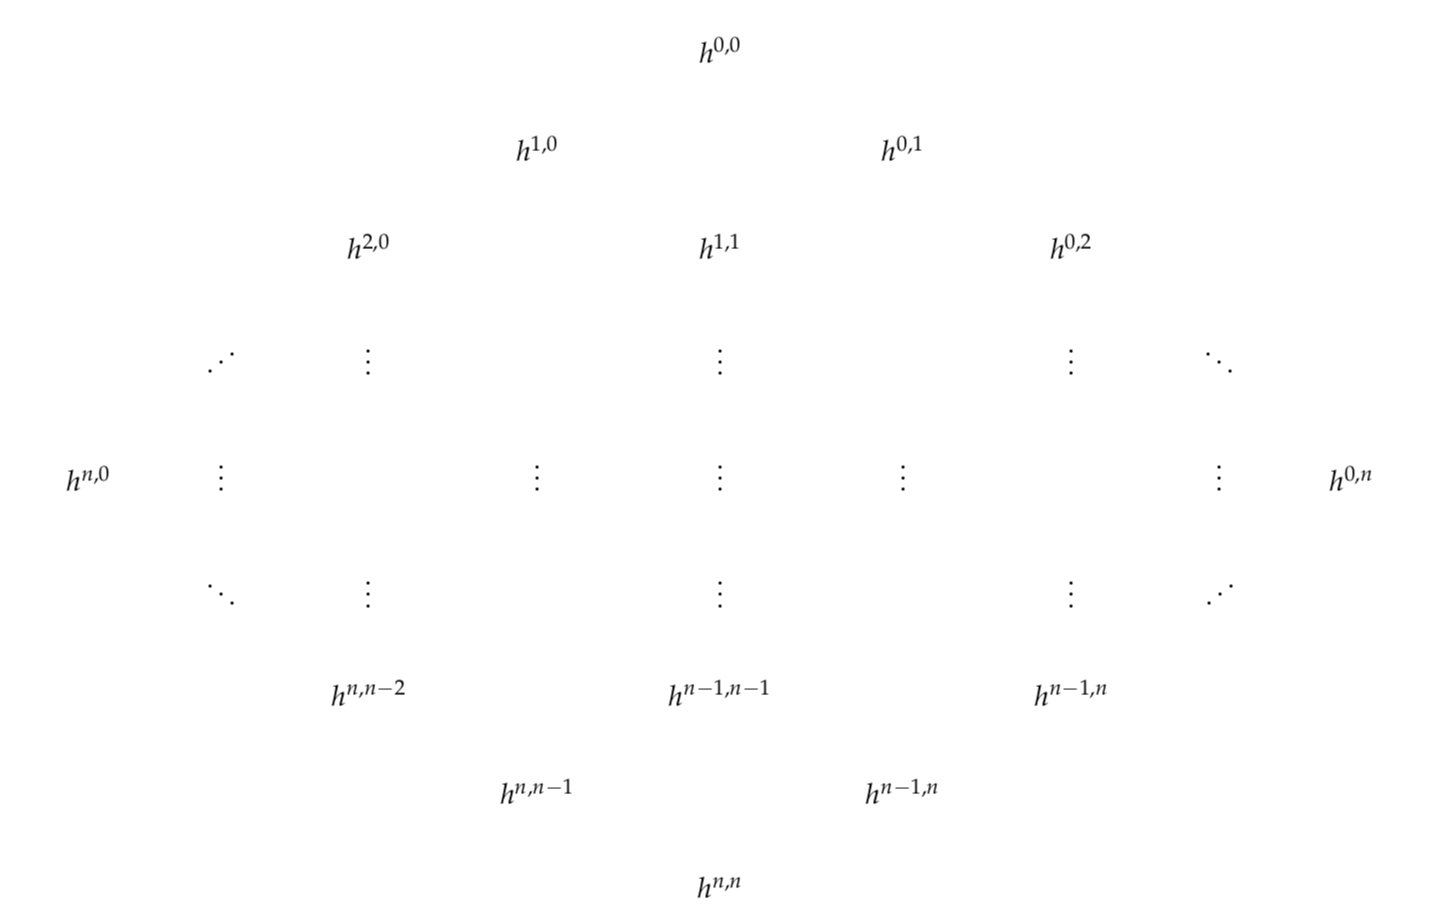
\includegraphics[width=\textwidth]{HodgeDiamond}
\end{figure}
\iffalse
\[\hspace*{-1.65cm}\begin{tikzcd}
&&&& h^{0,0}\\
&&& h^{1,0} & & h^{0,1}\\
&& h^{2,0} & & h^{1,1} & & h^{0,2} \\
&\iddots &  \vdots && \vdots && \vdots    & \ddots \\
h^{n,0} & \vdots && \vdots & \vdots & \vdots && \vdots & h^{0,n} \\
&\ddots & \vdots && \vdots && \vdots  & \iddots \\
&& h^{n,n-2} & & h^{n-1,n-1} & & h^{n-1,n} \\
&&& h^{n,n-1} & & h^{n-1,n} \\
&&&& h^{n,n}
\end{tikzcd}\]
\fi
We then see that our observations about the Hodge numbers are encoded in symmetries
of the Hodge diamond. Complex conjugation corresponds to  reflecting across the
vertical line of symmetry, so $h^{p,q} = h^{q,p}$ implies that the diamond is
symmetric across this line. The Hodge star gives us that $h^{p,q} = h^{n-p,n-q}$,
which corresponds to a reflection across the horizontal line of symmetry of the Hodge
diamond. Finally, Serre duality tells us that $h^{p,q} = h^{n+p,n-q}$, which
corresponds to a rotation of the Hodge diamond by $180$ degrees. These symmetries of
the Hodge diamond give another criterion for identifying complex
manifolds that do not admit a K\"ahler structure -- if we find a complex manifold
with a Hodge diamond that does not have the symmetries we listed above, then it cannot
be K\"ahler.
%
\section{The Hodge Index Theorem}
%
The Hodge Index theorem concerns the signature of an intersection form on a
K\"ahler manifold.
%
\begin{defn}
For a compact K\"ahler manifold $X$ of complex dimension $n$, let $L$ be the Lefschetz
operator on cohomology. Then for $k \leq n$, define the form $Q_k$ on $H^k(X,\R)$ by
\[
Q_k(\alpha,\beta) = \int_X \omega^{n-k}\wedge\alpha\wedge\beta
\]
\end{defn}
%
One thing to note is that if $k$ is even, then $\alpha$ and $\beta$ commute, so
$Q_k$ is symmetric. Otherwise, they anticommute, in which case $Q_k$ is antisymmetric.
%
\begin{defn}
Define the Hermitian forms $H_k : H^j(X,\C) \otimes \overline{H^j(X,\C)} \to \C$ by
\[
H_k(\alpha,\beta) = i^kQ_j(\alpha,\beta)
\]
\end{defn}
%
\begin{thm}
The Lefschetz decomposition on cohomology
\[
H^k(X,\C) = \bigoplus_{r\geq 0} L^r H^{k-2r}(X,\C)_{\mathrm{Prim}}
\]
is orthogonal with respect to the Hermitian form $H_k$. On each primitive component
$L^rH^{k-2r}(X,\C)_{\mathrm{Prim}}$ the form $H_k$ on $H^k(X,\C)$ induces the form
$(-1)^rH_{k-2r}$\footnote{In Voisin, the statement is, ``the form $H_r$ on $H^k(X,\C)$
induces\ldots," but appears to be a typo, as the computation will show}.
\end{thm}
%
\begin{proof}
Suppose $\alpha \in L^rH^{k-2r}(X,\C)$ and $\beta \in L^sH^{k-2s}(X,\C)$. We want to
show that $H_k(\alpha,\beta) = 0$. Write $\alpha = L^r\alpha'$ and $\beta = L^s\beta'$
with $\alpha'$ and $\beta'$ primitive, i.e. annihilated by $L^{n-k+2r+1}$ and
$L^{n-k+2s+1}$ respectively. WLOG, we may assume that $r < s$. Therefore, we compute
\begin{align*}
H_k(\alpha,\beta) &= H_k(L^r\alpha',L^s\beta') \\
&= i^kQ_k(L^r\alpha',\overline{L^s\beta'}) \\
&= i^k\int_X \omega^{n-k}\wedge\omega^r
\wedge\alpha'\wedge\overline{\omega^s\wedge\beta'} \\
&= i^k\int_X \omega^{n-k+r+s} \wedge \alpha'\wedge\overline{\beta'} \\
&= i^k\int_X L^{n-k+r+s}\alpha' \wedge \overline{\beta'}
\end{align*}
Then since $r < s$, we have $r+s > 2r$, and since $L^{n-k+2r+1}\alpha' = 0$, this
implies that $L^{n-k+r+s}\alpha' = 0$. Therefore, $H_k(\alpha,\beta) = 0$, proving
orthogonality. \\

For the second statement, we see that for
$L^r\alpha,L^r\beta \in L^rH^{k-2r}(X,\C)_{\mathrm{Prim}}$ we have
\begin{align*}
H_k(L^r\alpha,L^r\beta) &=
i^k\int_X \omega^{n-k}\wedge\omega^r\wedge\alpha\wedge\overline{\omega^r\wedge\beta} \\
&= i^k\int_X\omega^{n-k+2r}\wedge\alpha\wedge\overline{\beta} \\
&= i^k Q_{k-2r}(\alpha,\overline{\beta}) \\
\end{align*}
For comparison, we have that
\begin{align*}
(-1)^rH_{k-2r}(\alpha,\beta) &= (-1)^ri^{k-2r}Q_{k-2r}(\alpha,\overline{\beta}) \\
&= i^kQ_{k-2r}(\alpha,\overline{\beta})\\
\end{align*}
which shows the desired equality.
\end{proof}
%
Another orthogonality result:
%
\begin{thm}
The Hodge decomposition
\[
H^k(X,\C) = \bigoplus_{p+q=k} H^{p,q}(X,\C)
\]
is orthogonal with respect to the $H_k$.
\end{thm}
%
\begin{proof}
Let $(p,q) \neq (p',q')$ with $p+q = p'+ q' = k$, with $\alpha \in H^{p,q}(X,\C)$
and $\beta \in H^{p',q'}(X,\C)$. Then $L^{n-k}\alpha\wedge\overline{\beta}$
is of bidegree $(n-k+p+q',n-k+q+p')$. We note that this is of degree $2n$, but
is not of type $(n,n)$, since $(p,q) \neq (p',q')$. But $H^{2n}(X,\C) = H^{n,n}(X,\C)$,
since it is trivialized by the volume form $\omega^n$. Therefore, we must have
that $L^{n-k}\alpha\wedge\beta = 0$, and consequently, $H_k(\alpha,\beta) = 0$.
\end{proof}
%
For the next proposition, we first use a lemma.
%
\begin{lem}
Let $\alpha \in \Lambda^{p,q}T^*_xX$. be primitive, with $p+q=k$. Then
\[
\star\alpha = \frac{(-1)^{\frac{k(k+1)}{2}}i^{p-q}}{(n-k)!}L^{n-k}\alpha
\]
\end{lem}
%
the proof is a somewhat tedious computation -- we will use this lemma without proof.
%
\begin{prop}
The form
\[
(-1)^{\frac{k(k+1)}{2}}i^{p-q-k}H_k
\]
is positive definite on
$H^{p,q}_{\mathrm{Prim}} \defeq H^k(X,\C)_{\mathrm{Prim}} \cap H^{p,q}(X,\C)$.
\end{prop}
%
\begin{proof}
We use the identification of $H^{p,q}(X,\C)$ with the space $\mathcal{H}^{p,q}(X)$ of
harmonic forms, and $L$ with the Lefschetz operator on forms restricted to harmonic
forms. Since $L$ commutes with complex conjugation, using Lemma 10.5, we have that for
a harmonic form $\alpha \in \mathcal{H}^{p,q}(X)$,
\[
\star\overline{\alpha}
= \frac{(-1)^{\frac{k(k+1)}{2}}i^{p-q}}{(n-k)!}L^{n-k}\overline{\alpha}
\]
Therefore, we have that
\begin{align*}
H_k(\alpha,\alpha) &= i^k\int_X L^{n-k}\alpha \wedge \overline{\alpha} \\
&= i^k\int_X \alpha \wedge L^{n-k}\overline{\alpha} \\
&= (n-k)!(-1)^{\frac{k(k+1)}{2}}i^{q-p+k} \int_X a\wedge\star\overline{\alpha} \\
&= (n-k)!(-1)^{\frac{k(k+1)}{2}}i^{q-p+k} |\alpha|_{L^2}
\end{align*}
Therefore, we have that
\begin{align*}
(-1)^{\frac{k(k+1)}{2}}i^{p-q-k}H_k(\alpha,\alpha)
&= (-1)^{\frac{k(k+1)}{2}}i^{p-q-k}(n-k)
!(-1)^{\frac{k(k+1)}{2}}i^{q-p+k}|\alpha|_{L^2}\\
&= (-1)^{k(k+1)}i^{0}(n-k)!\norm{\alpha}_{L^2} \\
&= (n-k)!\norm{\alpha}_{L^2}
\end{align*}
which is clearly positive for $\alpha \neq 0$, so the form is positive definite.
\end{proof}
%
We now prove the Hodge Index Theorem.
%
\begin{thm}[\ib{The Hodge Index Theorem}]
For the intersection form
\begin{align*}
Q : H^n(X,\R) &\otimes H^n(X, \R) \to \R \\
(\alpha,\beta) &\mapsto \int_X \alpha \wedge \beta
\end{align*}
on a compact K\"ahler manifold $X$ of even complex dimension $n$, the signature
$\sigma(Q)$ is equal to
\[
\sigma(Q) = \sum_{a,b}(-1)^ah^{a,b}
\]
\end{thm}
%
\begin{proof}
Given a basis for $H^n(X,\R)$, this defines a basis for $H^n(X,\C)$ as a complex
vector space, and the intersection form $Q$ is represented by the same matrix as
the Hermitian form
\[
H(\alpha,\beta) = \int_X \alpha \wedge \overline{\beta}
\]
so it suffices to compute the signature of $H$. The Lefschetz decomposition gives
us a direct sum decomposition
\[
H^n(X,\C) = \bigoplus_{r\geq 0}L^rH^{n-2r}(X,\C)_{\mathrm{Prim}}
\]
which when combined with the Hodge decomposition, gives us
\[
H^n(X,\C) = \bigoplus_{r\geq 0, a+b+2r = n}L^rH^{a,b}(X,\C)_{\mathrm{Prim}}
\]
we then compute the signature on each component of the direct sum, and then sum them
together. By Theorem 10.3, we have that the form $H_n = i^nH$ induces
the form $(-1)^{a+b}H_{n-2(a+b)}$ on $L^rH^{a+b}(X, \C)_{\mathrm{Prim}}$.
\end{proof}





\iffalse
\begin{proof}
Fix holomorphic coordinates $z^1,\ldots z^n$ such that the Hermitian metric $h$ for
$X$ at $x$ is given by $h_x = \sum_i dz^id\zbar^i$. We can then uniquely write the
$\alpha$ in these coordinates as
\[
\alpha = \sum_{A,B,M}\gamma_{A,B,M} \omega_M \wedge dz^A\wedge dz^B
\]
where $\omega_M$ is the form
\[
\omega_M = dz^{i_1}\wedge d\zbar^{i_1}\wedge\cdots\wedge dz^{i_m}\wedge d\zbar^{i_m}
\]
as we defined in the proof of Proposition 8.1, and
$A,B$ and $M$ are are disjoint subsets of $\set{1,\ldots,n}$ where
$|A| + |B| + 2|M| = k$. Recall the identity
\[
\Lambda = -2i\sum_i \iota_{\partial_i \wedge \dbar_i}
\]
where
\begin{align*}
\partial_i &\defeq \frac{\partial}{\partial z^i} \\
\dbar_i &\defeq \frac{\partial}{\partial \zbar^i}
\end{align*}
which comes from the computation in Proposition 8.1. Using this identity, we compute
for fixed $A,B,M$
\begin{align*}
\Lambda(\omega_M \wedge dz^A\wedge d\zbar^B)
&= -2i\sum_i \iota_{\partial_i\wedge\dbar_i}(\omega_M \wedge dz^A\wedge d\zbar^B)
\end{align*}
Noting that the term
$\iota_{\partial_i\wedge\dbar_i}(\omega_M \wedge dz^A\wedge d\zbar^B)$ is nonzero
only when $i \in M$, we obtain
\[
\Lambda(\omega_M \wedge dz^A\wedge d\zbar^B)
= -2i\sum_{i\in M}\omega_{M - \set{i}}\wedge dz^A\wedge d\zbar^B
\]
Since $\alpha$ is primitive, we have that
\begin{align*}
0 = \Lambda\alpha
&= \sum_{A.B,M}\gamma_{A,B,M}\Lambda(\omega_M\wedge dz^A\wedge d\zbar^B) \\
&= -2i\sum_{A,B,M}\sum_{i \in M}
\gamma_{A,B,M}\omega_{M - \set{i}}\wedge dz^A\wedge d\zbar^B
\end{align*}
Let $\alpha_{A,B} = \sum_M\gamma_{A,B,M}\omega_M\wedge dz^A\wedge d\zbar^B$, so
$\alpha = \sum_{A,B}\alpha_{A,B}$. A slightly tricky verification reveals that
$\Lambda\alpha_{A,B}$ must also vanish (the verification involves checking the
$dz^i$ and $d\zbar^i$ contained in each term to show that they are distinct). Therefore,
all the $\alpha_{A,B}$ are primitive, and verifying the identity on the $\alpha_{A,B}$
verifies it on $\alpha$ by linearity. For slightly cleaner notation,
rewrite $\alpha_{A,B}$ as
$\alpha_{A,B} = \left(\sum_M \gamma_M\omega_M\right) \wedge dz^A\wedge d\zbar^B$.
Then since $\Lambda\alpha_{A,B} = 0$, we have that for any subset
$N \subset \set{1,\ldots, n}$ disjoint from $A \cup B$ of cardinality $|M| - 1$,
\[
\sum_{i \in \set{1,\ldots,n}-(A \cup B \cup N)} \gamma_{N\cup\set{i}} = 0
\]
we claim that this condition implies the following:
\begin{claim}
For any fixed $J \subset \set{1,\ldots n} - (A \cup B)$ such that
$|J| = n - |A| - |B| - |M|$
\[
\sum_{N \subset J}\gamma_N = (-1)^{|M|}\gamma_{\set{1,\ldots,n}-(A\cup B\cup J)}
\]
where we sum over subsets $N$ where $|N| = |M|$.
\end{claim}
\end{proof}
\fi
%
\newpage
%
\nocite{*}
%
\printbibliography
%
\end{document}